\documentclass[11pt,a4paper]{amsart}
\usepackage[T1]{fontenc}
\usepackage[utf8]{inputenc}
\usepackage[british]{babel}
\usepackage{lmodern,microtype}
\usepackage[margin=28.8mm]{geometry}
\usepackage{amsmath,amssymb,amsthm,mathtools}
\usepackage{graphicx,booktabs,tabularx,array,longtable}
\usepackage[dvipsnames]{xcolor}
\usepackage{tikz,pgfplots,helvet}
\pgfplotsset{compat=1.18}
\usepackage{algorithm,algpseudocode,capt-of}
\usepackage[section]{placeins}
\usepackage[numbers]{natbib}
\usepackage{xurl}
\urlstyle{same}
\usepackage[colorlinks=true,linkcolor=MidnightBlue,citecolor=MidnightBlue,urlcolor=MidnightBlue]{hyperref}
\providecommand{\algorithmautorefname}{Algorithm}
% amsart's table-of-contents reader also takes the list title.
\makeatletter
\newswitch{loa}
\let\l@algorithm\l@figure
\renewcommand{\listofalgorithms}{\@starttoc{loa}{\listalgorithmname}}
\makeatother
% Editable reconstructions of the three figures in the supplied PDF.
% The source PDF contains vector plots but no original plotting source.
% Coordinates below preserve its 432 bp-wide canvases, colours, and scales.
% Only \usepackage{tikz} is required; no external graphics or shell escape.
% Helvetica/Nimbus Sans replaces the PDF's embedded DejaVu Sans font.

\definecolor{EWOink}{RGB}{32,48,56}
\definecolor{EWOteal}{RGB}{0,124,131}
\definecolor{EWOrust}{RGB}{170,75,34}
\definecolor{EWOgrey}{RGB}{91,102,106}
\definecolor{EWOagent}{RGB}{98,107,117}
\definecolor{EWOgrid}{RGB}{199,205,208}
\newcommand{\PaperFigureFont}{\fontfamily{phv}\selectfont}
\tikzset{
  ewo figure/.style={x=1bp,y=1bp,line cap=butt,line join=round,
    every node/.style={anchor=base west,inner sep=0pt,outer sep=0pt,
      text=EWOink,font=\PaperFigureFont\fontsize{8.5bp}{10bp}\selectfont}},
  ewo title/.style={font=\PaperFigureFont\bfseries\fontsize{11bp}{13bp}\selectfont},
  ewo label/.style={font=\PaperFigureFont\fontsize{9bp}{11bp}\selectfont},
  ewo panel/.style={font=\PaperFigureFont\fontsize{10bp}{12bp}\selectfont},
  ewo axis/.style={draw=EWOgrey,line width=.6bp},
  ewo tick/.style={draw=EWOink,line width=.6bp}
}

\newcommand{\AttemptTimelineFigure}{%
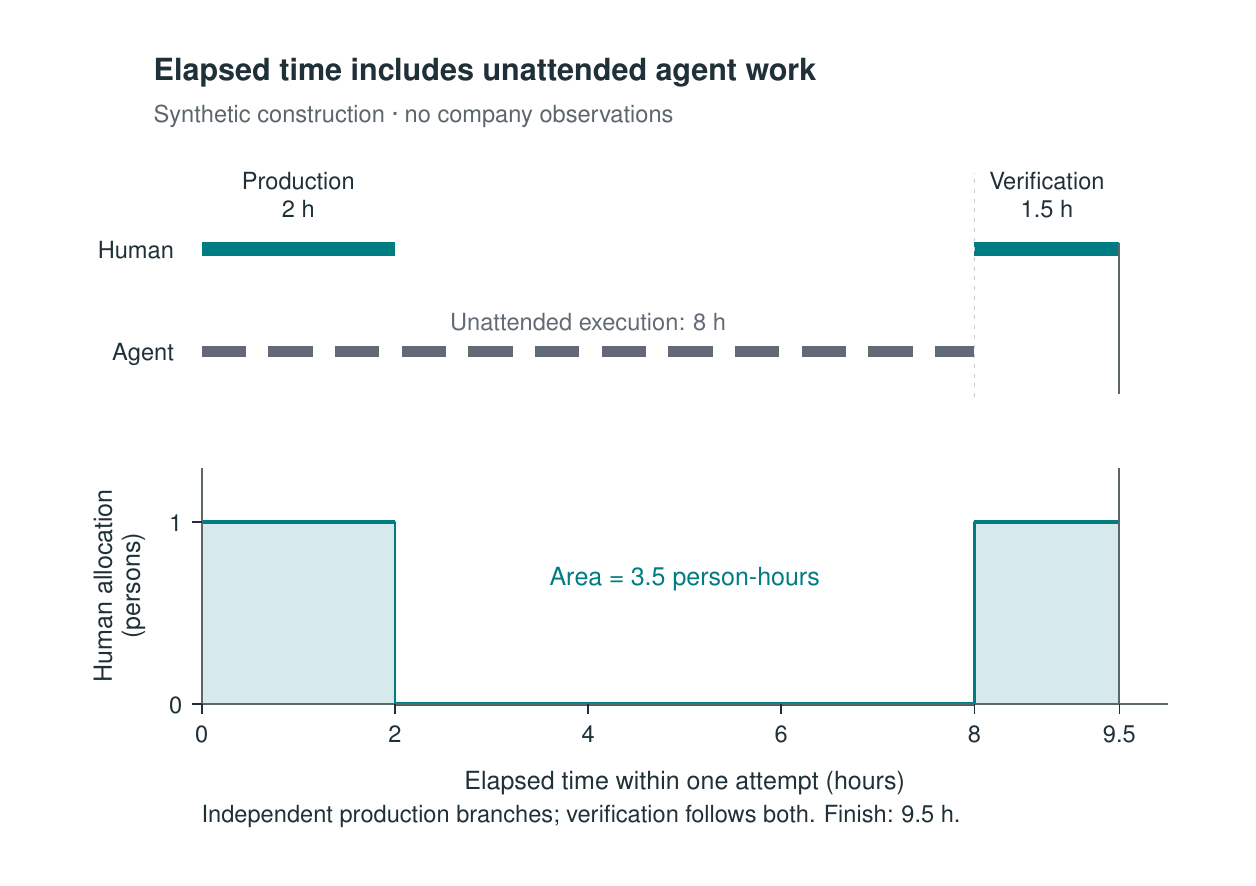
\begin{tikzpicture}[ewo figure]
  \path[use as bounding box] (0,0) rectangle (432,298.8);
  \node[ewo title] at (45.36,279.684)
    {Elapsed time includes unattended agent work};
  \node[text=EWOgrey] at (45.36,264.765)
    {Synthetic construction \textperiodcentered\ no company observations};

  % Independent branches: c_h=2 h, g=8 h, followed by v=1.5 h.
  % Both panels use x = 62.64 + 34.776 * elapsed hours.
  \node[anchor=base east] at (52.64,215.585) {Human};
  \node[anchor=base east] at (52.64,178.914) {Agent};
  \draw[EWOteal,line width=5bp] (62.64,219.007)--(132.192,219.007);
  \draw[EWOteal,line width=5bp] (340.848,219.007)--(393.012,219.007);
  \draw[EWOagent,line width=4bp,dash pattern=on 16bp off 8bp]
    (62.64,182.336)--(340.848,182.336);
  \draw[EWOgrid,line width=.7bp,dash pattern=on 1.4bp off 2.1bp]
    (340.848,165.834)--(340.848,246.51);
  \draw[EWOgrey,line width=.7bp] (393.012,166.934)--(393.012,221.207);
  \node[anchor=base] at (97.416,240.504) {Production};
  \node[anchor=base] at (97.416,230.416) {2 h};
  \node[anchor=base] at (366.93,240.504) {Verification};
  \node[anchor=base] at (366.93,230.416) {1.5 h};
  \node[anchor=base,text=EWOagent] at (201.744,189.670)
    {Unattended execution: 8 h};

  % Human allocation is one person on [0,2] and [8,9.5], zero otherwise.
  \fill[EWOteal,opacity=.16] (62.64,55.278) rectangle (132.192,120.784);
  \fill[EWOteal,opacity=.16] (340.848,55.278) rectangle (393.012,120.784);
  \draw[EWOteal,line width=.8bp]
    (62.64,55.278)--(62.64,120.784)--(132.192,120.784)--(132.192,55.278)
    (340.848,55.278)--(340.848,120.784)--(393.012,120.784)--(393.012,55.278);
  \draw[EWOteal,line width=1.5bp]
    (62.64,120.784)--(132.192,120.784)
    (132.192,55.278)--(340.848,55.278)
    (340.848,120.784)--(393.012,120.784);
  \draw[EWOgrey,line width=.7bp] (393.012,55.278)--(393.012,140.436);
  \draw[ewo axis] (62.64,140.436)--(62.64,55.278)--(410.4,55.278);
  \foreach \hour in {0,2,4,6,8,9.5}{
    \draw[ewo tick] ({62.64+34.776*\hour},55.278)--++(0,-3.5);
    \node[anchor=base] at ({62.64+34.776*\hour},41.434) {\hour};
  }
  \foreach \allocation in {0,1}{
    \draw[ewo tick] (62.64,{55.278+65.506154*\allocation})--++(-3.5,0);
    \node[anchor=base east] at (55.64,{51.856+65.506154*\allocation})
      {\allocation};
  }
  \node[ewo label,anchor=base,rotate=90] at (30.271,97.857) {Human allocation};
  \node[ewo label,anchor=base,rotate=90] at (40.359,97.857) {(persons)};
  \node[ewo label,anchor=base] at (236.52,24.716)
    {Elapsed time within one attempt (hours)};
  \node[ewo label,anchor=base,text=EWOteal] at (236.52,97.857)
    {Area = 3.5 person-hours};
  \node at (62.64,12.550)
    {Independent production branches; verification follows both. Finish: 9.5 h.};
\end{tikzpicture}%
}

\newcommand{\DetectionFigure}{%
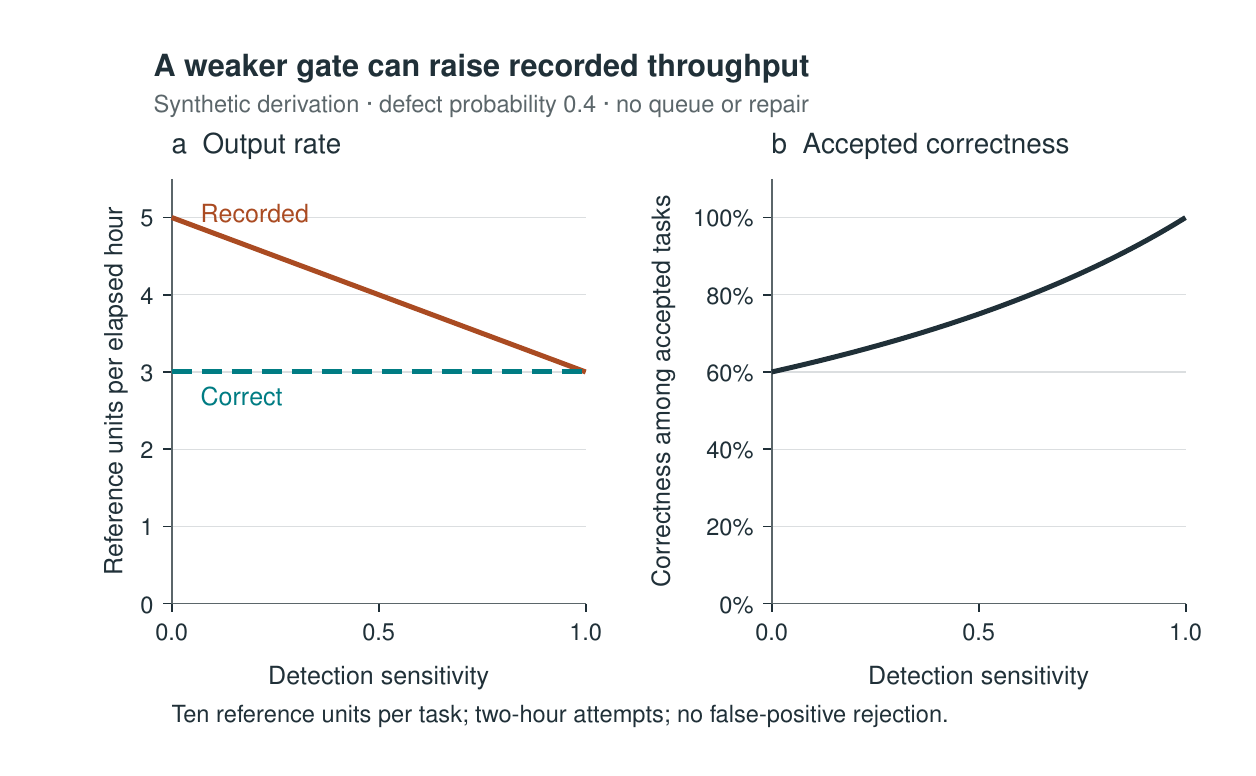
\begin{tikzpicture}[ewo figure]
  \path[use as bounding box] (0,0) rectangle (432,259.2);
  \node[ewo title] at (45.36,241.509)
    {A weaker gate can raise recorded throughput};
  \node[text=EWOgrey] at (45.36,228.769)
    {Synthetic derivation \textperiodcentered\ defect probability 0.4
     \textperiodcentered\ no queue or repair};
  \node[ewo panel] at (51.84,213.768) {a\ \ Output rate};
  \node[ewo panel] at (267.84,213.768) {b\ \ Accepted correctness};

  % Both axes: x in [0,1], left rate in [0,5.5], right fraction in [0,1.1].
  \foreach \xorigin in {51.84,267.84}{
    \foreach \step in {0,...,5}{
      \draw[EWOgrid,line width=.45bp,opacity=.65]
        (\xorigin,{51.84+27.805091*\step})--++(149.04,0);
      \draw[ewo tick] (\xorigin,{51.84+27.805091*\step})--++(-3,0);
    }
    \draw[ewo axis] (\xorigin,204.768)--(\xorigin,51.84)--++(149.04,0);
    \foreach \s/\ticktext in {0/0.0,0.5/0.5,1/1.0}{
      \draw[ewo tick] ({\xorigin+149.04*\s},51.84)--++(0,-3);
      \node[anchor=base] at ({\xorigin+149.04*\s},38.496) {\ticktext};
    }
    \node[ewo label,anchor=base] at ({\xorigin+74.52},22.778)
      {Detection sensitivity};
  }
  \foreach \step in {0,...,5}{
    \node[anchor=base east] at (45.34,{48.418+27.805091*\step}) {\step};
  }
  \foreach \step/\ticktext in {0/0,1/20,2/40,3/60,4/80,5/100}{
    \node[anchor=base east] at (261.34,{48.418+27.805091*\step}) {\ticktext\%};
  }
  \node[ewo label,anchor=base,rotate=90] at (34.059,128.304)
    {Reference units per elapsed hour};
  \node[ewo label,anchor=base,rotate=90] at (231.168,128.304)
    {Correctness among accepted tasks};

  % S^0=10, t=2, d=.4: recorded=5-2s; correct=3; rho=.6/(1-.4s).
  \draw[EWOrust,line width=1.8bp]
    plot[domain=0:1,samples=2] ({51.84+149.04*\x},{51.84+27.805091*(5-2*\x)});
  \draw[EWOteal,line width=1.8bp,dash pattern=on 7.2bp off 3.6bp]
    (51.84,135.255273)--(200.88,135.255273);
  \draw[EWOink,line width=1.8bp]
    plot[domain=0:1,samples=101] ({267.84+149.04*\x},{51.84+139.025455*(.6/(1-.4*\x))});
  \node[ewo label,text=EWOrust] at (62.273,188.919) {Recorded};
  \node[ewo label,text=EWOteal] at (62.273,123.299) {Correct};
  \node at (51.84,9.072)
    {Ten reference units per task; two-hour attempts; no false-positive rejection.};
\end{tikzpicture}%
}

\newcommand{\EffortTimeFigure}{%
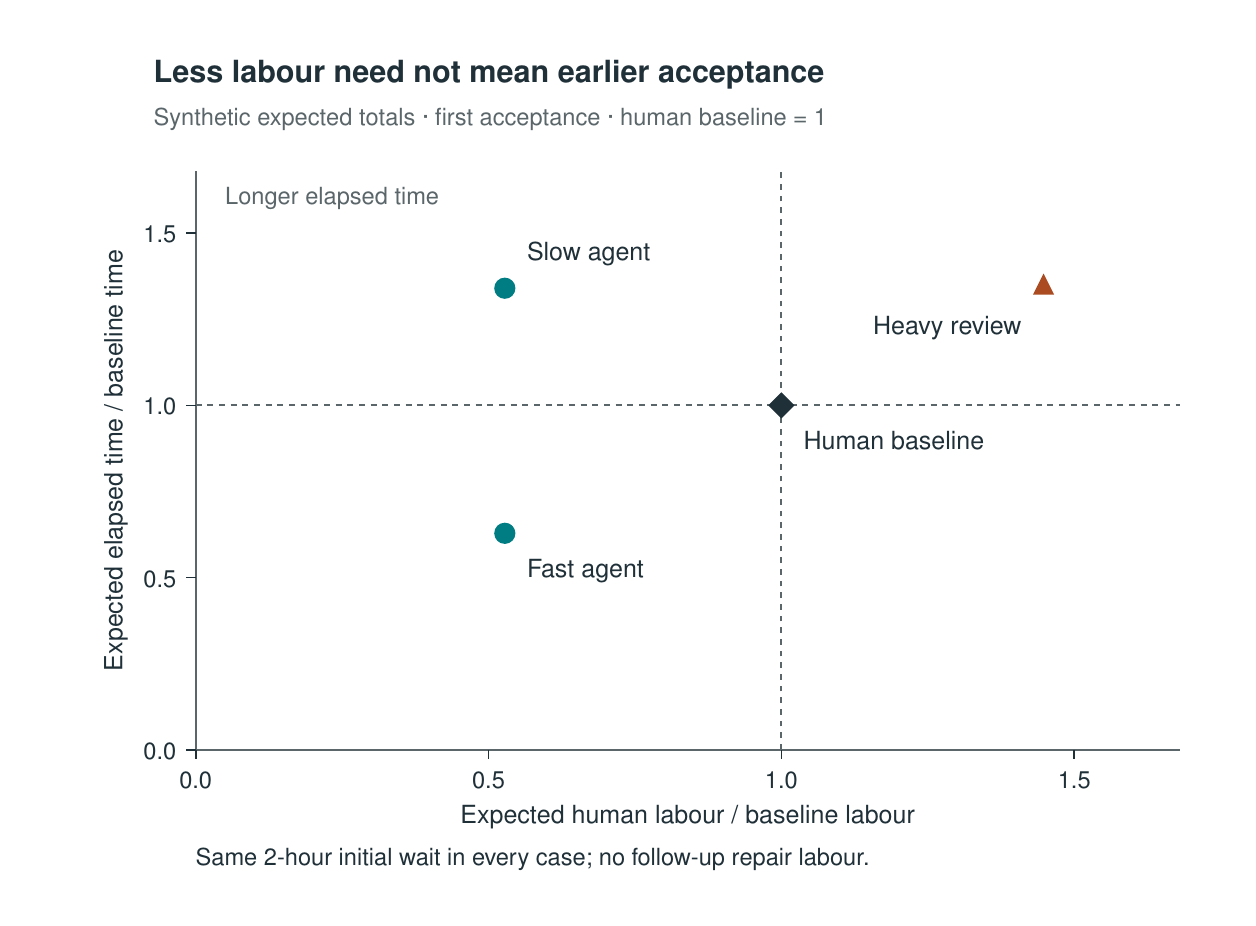
\begin{tikzpicture}[ewo figure]
  \path[use as bounding box] (0,0) rectangle (432,313.2);
  \node[ewo title] at (45.36,293.565)
    {Less labour need not mean earlier acceptance};
  \node[text=EWOgrey] at (45.36,277.855)
    {Synthetic expected totals \textperiodcentered\ first acceptance
     \textperiodcentered\ human baseline = 1};

  % Ratios of E[H^A]=h/p and E[L]=2+t/p to the human baseline.
  % Plot scales: x=60.48+210.857142857*r_H, y=53.244+123.975*r_L.
  \draw[ewo axis] (60.48,261.522)--(60.48,53.244)--(414.72,53.244);
  \foreach \value/\ticktext in {0/0.0,0.5/0.5,1/1.0,1.5/1.5}{
    \draw[ewo tick] ({60.48+210.857142857*\value},53.244)--++(0,-3.5);
    \node[anchor=base] at ({60.48+210.857142857*\value},39.400) {\ticktext};
    \draw[ewo tick] (60.48,{53.244+123.975*\value})--++(-3.5,0);
    \node[anchor=base east] at (53.48,{49.822+123.975*\value}) {\ticktext};
  }
  \draw[EWOgrey,line width=.7bp,dash pattern=on 2.1bp off 2.1bp]
    (271.337143,53.244)--(271.337143,261.522)
    (60.48,177.219)--(414.72,177.219);
  \node[ewo label,anchor=base] at (237.6,26.682)
    {Expected human labour / baseline labour};
  \node[ewo label,anchor=base,rotate=90] at (34.089,157.383)
    {Expected elapsed time / baseline time};
  \node[text=EWOgrey] at (71.107,249.471) {Longer elapsed time};

  % Baseline: h=t=7, p=.95; fast: h=t=3.5, p=.9;
  % slow: h=3.5,t=9.5,p=.9; review: h=t=8,p=.75.
  \pgfmathsetmacro{\ewobaselineH}{7/.95}
  \pgfmathsetmacro{\ewobaselineL}{2+7/.95}
  \pgfmathsetmacro{\ewofastX}{60.48+210.857142857*(3.5/.9)/\ewobaselineH}
  \pgfmathsetmacro{\ewofastY}{53.244+123.975*(2+3.5/.9)/\ewobaselineL}
  \pgfmathsetmacro{\ewoslowY}{53.244+123.975*(2+9.5/.9)/\ewobaselineL}
  \pgfmathsetmacro{\eworeviewX}{60.48+210.857142857*(8/.75)/\ewobaselineH}
  \pgfmathsetmacro{\eworeviewY}{53.244+123.975*(2+8/.75)/\ewobaselineL}
  \fill[EWOink] (271.337143,172.528584)--(276.027559,177.219)
    --(271.337143,181.909416)--(266.646727,177.219)--cycle;
  \fill[EWOteal] (\ewofastX,\ewofastY) circle[radius=3.817bp];
  \fill[EWOteal] (\ewofastX,\ewoslowY) circle[radius=3.817bp];
  \fill[EWOrust] (\eworeviewX,{\eworeviewY+3.817})
    --({\eworeviewX-3.817},{\eworeviewY-3.817})
    --({\eworeviewX+3.817},{\eworeviewY-3.817})--cycle;
  \node[ewo label] at (279.337143,161.219) {Human baseline};
  \node[ewo label] at ({\ewofastX+8},{\ewofastY-16}) {Fast agent};
  \node[ewo label] at ({\ewofastX+8},{\ewoslowY+10}) {Slow agent};
  \node[ewo label,anchor=base east] at ({\eworeviewX-8},{\eworeviewY-18})
    {Heavy review};
  \node at (60.48,11.588)
    {Same 2-hour initial wait in every case; no follow-up repair labour.};
\end{tikzpicture}%
}

\newtheorem{proposition}{Proposition}[section]
\newtheorem{corollary}[proposition]{Corollary}
\theoremstyle{definition}
\newtheorem{example}[proposition]{Example}
\theoremstyle{remark}
\newtheorem{remark}[proposition]{Remark}
\newcommand{\E}{\mathbb E}
\newcommand{\Prb}{\mathbb P}
\newcommand{\Var}{\operatorname{Var}}
\newcommand{\Cov}{\operatorname{Cov}}
\newcommand{\Corr}{\operatorname{Corr}}
\newcommand{\ind}{\mathbf 1}
\title[What software-work telemetry identifies]{What software-work telemetry identifies:\newline sharp labour bounds and design-based estimation}
\date{Methodological draft, 29 October 2026}
\keywords{software engineering, partial identification, labour bounds, activity sampling, model-assisted estimation, AI assistance}
\begin{document}
\begin{abstract}
Software-work telemetry records events whose relationship to human labour can change under AI assistance. We determine what labour is identified by specified observations, while keeping elapsed time to acceptance and retained output as separate endpoints. Exact interval totals and a per-person capacity constraint yield attainable labour bounds at a requested cutoff. For overlapping observations and shared capacity, partitioning time at observation endpoints and target cutoffs reduces the continuous allocation problem exactly to a finite linear programme. Its extrema give sharp bounds conditional on the declared observations; separate interval bounds can be wider. When labour is probability-sampled, fixed telemetry predictions can assist estimation through a design-unbiased residual correction. Its variance depends on prediction residuals, so inaccurate predictions can reduce precision. A marked-history representation keeps deadline acceptance, delayed retention assessment and fixed-horizon labour on their respective clocks without assuming Markov dynamics or independent attempts. We connect these results to a proposed cluster-randomised measurement pilot. The contribution is an observation-to-estimand specification with analytical proofs and finite computational checks. No organisational data are analysed, empirical calibration remains open, and the new results do not extend the retained historical Lean proof coverage.
\end{abstract}
\maketitle

\section{What the observations determine}
\label{sec:introduction}

Suppose a team records three person-hours of work during a four-hour interval. How much occurred during its first two hours? If one person supplied the work, the answer lies between one and two person-hours: at most two fit after the cutoff, and at most two fit before it. Both limits are attainable. The interval total therefore identifies a range without identifying the allocation within it. Commit times alone may supply even less information, because the same event sequence can arise from different amounts of human activity.

This article develops that observation-to-estimand argument for AI-assisted software work. The targets are all-role person-hours, elapsed time to first acceptance and reference output retained at a stated follow-up. Their definitions preserve unsuccessful work, concurrent activity and post-acceptance repair. The principal result shows that exact interval observations and shared per-person capacity constraints admit an exact finite linear-programming representation of all feasible labour totals. Minimising and maximising the desired total gives sharp bounds: every value between the extrema is attainable by an admissible allocation. Sharpening these bounds is consequently a question about additional observations or justified restrictions, rather than a choice of interpolation convention.

Probability sampling supplies a different kind of information. When exact allocation totals are unavailable, known inclusion probabilities support design-unbiased labour estimates. Fixed predictions from telemetry can improve their precision through a residual correction, but only when the residuals have a favourable variance under the sampling design. The same telemetry can therefore be insufficient to identify labour by itself and useful as an auxiliary predictor when independent allocation observations are available. We keep deterministic identification intervals, sampling uncertainty and uncertainty in a causal policy contrast distinct.

Wright and Ziegler's Standard Coder approach \cite{wright2019} motivates the observation problem. It infers coding activity from commit timing and predicts the resulting labels from code-change features. Standard Coding Hours (SCH) can serve as a common reference index, but calibration to independently observed labour requires a separate argument. AI may alter both the event-to-activity relationship and the work represented by a code change. The SPACE framework already places activity and efficiency within a broader account of developer productivity \cite{forsgren2021}; the CUPS taxonomy examines interaction time costs in AI-assisted programming \cite{mozannar2024}. Our narrower contribution is the labour identified or estimable under an explicit observation scheme, together with compatible timing and retained-output endpoints.

Existing AI studies also show why those endpoints matter. Peng et al.\ examine completion time among completers of a programming exercise \cite{peng2023}; Becker et al.\ study experienced maintainers in familiar repositories with a forecast-adjusted log-time contrast \cite{becker2025}; and Cui et al.\ study weekly completed pull requests in organisational experiments \cite{cui2026}. The latter's June 2025 manuscript uses assignment as an instrument for adoption \cite[Section 4.1 and Table 3]{cui2025manuscript}. Their populations, interventions and outcomes differ. METR's subsequent account of selection and concurrent-agent measurement difficulties further motivates separate labour and elapsed-time records \cite{metr2026}. These studies supply context, not interchangeable parameters or data for the calculations here.

Sections~\ref{sec:observation} and~\ref{sec:accounting} define the observation problem and endpoints. Section~\ref{sec:sharp-identification} derives the labour bounds, and Section~\ref{sec:estimation} connects sampled labour to telemetry-assisted estimation. Section~\ref{sec:study} gives a prospective protocol that could assess the measurements before estimating a policy effect. The finite reduction and attainability arguments specialise standard optimisation and sampling ideas to the stated allocation constraints; no new probability theory is claimed. Illustrative execution mechanisms, targeted Standard Coder corrections and a measured implementation comparison appear in the appendices. The implementation comparison concerns repeated discrete accounting queries, not the cost of solving the sharp-bounds programme or the productivity of a software team.

\section{Why event telemetry alone need not identify labour}
\label{sec:observation}

Let a minute-indexed hidden variable $Z_t\in\{0,1\}$ indicate an activity state, and let $C_t\in\{0,1\}$ record a commit event. A fitted event model specifies both activity dynamics and an emission mechanism. Calling $Z_t=1$ ``coding'' supplies a semantic interpretation, but it does not establish that the state equals independently measured labour. Moreover, the same event law can arise from different activity laws.

\begin{proposition}[Failure of unrestricted identification]
\label{prop:nonidentification}
Suppose the states $Z_t$ are independent Bernoulli variables with parameter $\pi\in(0,1)$, and, independently across minutes and of the states, $B_t$ are Bernoulli variables with parameter $c\in(0,1)$. Define $C_t=Z_tB_t$. The complete law of the event process depends on $(\pi,c)$ only through $\pi c$. In particular, $(\pi,c)=(1/2,1/5)$ and $(1/4,2/5)$ give identical observed laws but different expected active times.
\end{proposition}

\begin{proof}
Each $C_t$ is Bernoulli with parameter $\theta=\pi c$, and the $C_t$ are independent. For every $n\geq1$ and every binary string $(e_1,\ldots,e_n)$,
\begin{equation}
\label{eq:event-law}
 \Prb(C_1=e_1,\ldots,C_n=e_n)
 =\theta^{\sum_t e_t}(1-\theta)^{n-\sum_t e_t}.
\end{equation}
Both parameter pairs give $\theta=1/10$. In contrast,
\begin{equation}
\label{eq:activity-total}
 \E\!\left[\sum_{t=1}^{n}Z_t\right]=n\pi,
\end{equation}
which is $n/2$ minutes in the first model and $n/4$ in the second. Thus the same observable distribution corresponds to two different target values.
\end{proof}

This construction belongs to the independent-state subfamily of a two-state hidden Markov model: both transition rows give the same next-state probability. It shows that the unrestricted family is not globally identifiable. Persistent or otherwise restricted models may still be identifiable. Additional restrictions, informative code marks or independent activity observations may distinguish the relevant cases. A guarantee must state which of those restrictions or observations supplies the information. AI makes the question more immediate because commit production can continue while human attention is elsewhere.

The appropriate next step is to specify what additional observations constrain labour. Internal agreement between model predictions cannot supply that information; Appendix~\ref{app:audit} states the limitation of a conditional-expectation consistency diagnostic.

\section{Task accounting with explicit boundaries}
\label{sec:accounting}

\subsection{The task, the policy and the person-hour}

Enrol task $i$ at time $s_i$, when its requested behaviour, eligibility and acceptance criteria are recorded. Task identity follows the requirement, rather than a commit or pull request. Before observing outcomes, define how split tasks, merged tasks and scope changes will be handled. A parent requirement can retain its original identity while children record implementation activity. Counting both the parent and its children as delivered output would count the same work twice. Material changes of scope require a versioned record and a stated analysis rule.

That rule must also fix task granularity, acceptance credit and the follow-up clock before policies are compared. Even additive reference scores can yield different deadline output when separately accepted components are regrouped into a parent accepted only after its last component. Freezing the score alone therefore leaves part of the comparison unspecified.

An \emph{AI policy} specifies which tools and model versions are available and which tasks are eligible. It also sets the permitted autonomy, review responsibilities and release rules. Assignment to this policy is the intervention in the proposed experiment. Actual exposure remains a recorded behaviour, since difficult tasks may elicit more use and people may decline an assigned tool.

Let $a_{ijr}(t)$ be the fraction of person $j$'s time allocated to task $i$ in role $r$ at time $t$. For a finite set of observed people, measurable allocation functions satisfy
\begin{equation}
\label{eq:labour}
 a_{ijr}(t)\geq0,\qquad \sum_{i,r}a_{ijr}(t)\leq1,\qquad
 H_i(u)=\sum_{j,r}\int_{s_i}^{s_i+u}a_{ijr}(t)\,dt.
\end{equation}
With time in hours, $H_i(u)$ has units of person-hours. Roles include specification, implementation, prompting, review, testing, integration and repair. Pair work can contribute two person-hours in one elapsed hour. Conversely, a person's two concurrent sessions cannot each receive a full hour of that person's attention. State whether attended waiting belongs in the labour total. Unattended execution is recorded as agent resource use.

Equation~\eqref{eq:labour} defines the target, while the observation procedure determines how precisely its allocations are known. Shared review and platform work therefore need an attribution rule, with an overhead category where allocation to tasks is indefensible. Record agent instance-hours by resource class, tokens and charges separately from person-hours. Combining these resources requires an explicit economic conversion and changes the question from labour to cost.

Let $T_i$ be elapsed time from enrolment to first acceptance. Starting this clock at enrolment includes queueing and any reasoning and specification between enrolment and the first commit. If the task is permanently abandoned before acceptance, put $T_i=\infty$. Abandonment is an outcome, whereas loss of observation is censoring. Record deployment separately whenever acceptance and deployment differ.

\subsection{A frozen reference and a follow-up assessment}

Assign a nonnegative reference score $S_i^0$ using a declared version and representation. It may count tasks, independent functional units or frozen SCH weights. A labour-calibrated reference would target
\begin{equation}
\label{eq:reference}
 S^0(x)=\E[H^{\mathrm{ref}}\mid X=x]
\end{equation}
for a specified reference population, resource boundary, quality bar and stopping rule, provided the expectation is finite. A predictor trained only on imputed coding labels targets those labels. Its calibration to independently measured labour requires a separate empirical test. The superscript $0$ denotes a fixed reference, not current effort under the intervention.

For a fixed-scope causal comparison, requirements recorded at intake are preferable to final code differences: AI can change the latter. A retrospective code score can still be reported, with its dependence on the implementation made explicit. Splitting and squashing also matter because a nonlinear scoring rule need not be additive. Score a canonical task representation once, or use an additive requirement rubric. A failed attempt, retry or revert must not generate another unit of retained output.

Choose an acceptance horizon $\tau>0$ and a follow-up duration $\Delta\geq0$. For accepted tasks, let $R_i(\Delta)\in[0,1]$ be the assessed fraction of the accepted requirement still meeting the rubric at time $s_i+T_i+\Delta$. Retained reference output is
\begin{equation}
\label{eq:retention}
 Q_i(\tau,\Delta)=\begin{cases} S_i^0 R_i(\Delta),&T_i\leq\tau,\\ 0,&T_i>\tau.\end{cases}
\end{equation}
The rubric must distinguish an intentional replacement from a defect-driven loss and explain fractional scores. Surviving lines, successful tests and absence of recorded incidents are observations of quality. None establishes complete correctness. Reliability of the assessment itself therefore belongs in the study.

For a finite intake cohort with positive total labour, define
\begin{equation}
\label{eq:cohort-productivity}
 P_H(\tau,\Delta)
 =\frac{\sum_i Q_i(\tau,\Delta)}{\sum_i H_i(\tau+\Delta)}.
\end{equation}
The denominator is the cohort's resource total through the fixed enrolment horizon. It includes labour on rejected, unfinished and abandoned tasks, together with task-attributable work after acceptance. An early acceptance leaves more of this horizon remaining than a late one. Stopping each task's repair accounting exactly $\Delta$ after acceptance therefore defines a different labour boundary. Either convention can be useful, but the choice must be explicit. Follow every enrolment for $\tau+\Delta$ to ascertain the numerator and this denominator.

A calendar-window rate answers another question. For a window $W$ of positive length and a defined portfolio of tasks, let
\begin{equation}
\label{eq:calendar-throughput}
 V_W=\frac{\sum_{i:\,s_i+T_i\in W}S_i^0R_i(\Delta)}{|W|}.
\end{equation}
All counted acceptances need the same subsequent follow-up. Record work in progress at the window boundaries because some output may have begun earlier. Dividing portfolio output by the sum of overlapping task durations gives neither this calendar rate nor a team's capacity. Zero-effort tasks do not require individual output/effort ratios. A positive aggregate denominator and the count of such tasks are sufficient.

\subsection{The observations and the three clocks}
\label{sec:event-history}

The endpoints use three observation times: acceptance is assessed against the deadline $\tau$, retention at task age $T_i+\Delta$, and labour through task age $\tau+\Delta$. Calculating these endpoints from a complete history requires no assumption of Markov dynamics or independent attempts. The acceptance event alone leaves subsequent loss and repair unresolved. A realised labour total is point-identified by a record when every admissible history consistent with that record gives the same total. Point identification here concerns a realised total. Proposition~\ref{prop:nonidentification} instead concerns a population parameter and the probability law of observations. We now derive the smallest and largest labour totals compatible with interval observations.


\section{Attainable labour ranges from interval observations}
\label{sec:sharp-identification}

An interval total leaves the timing of attention within it unresolved. We therefore seek all values of fixed-horizon labour compatible with the observations and the allocation constraint in \eqref{eq:labour}. The \emph{identified range} contains exactly those values: each is attained by at least one compatible history, and every compatible history gives a value in the range. This use of compatibility follows the general partial-identification perspective \cite[Section~1]{torgovitsky2019}. We prove the allocation results directly. They describe what the observations determine, with sampling uncertainty and causal intervention effects requiring separate analyses.

\subsection{Bounding labour at a bin boundary}
\label{sec:binning-bounds}

Exact bin masses can bound the continuous labour target even when the distribution of work within each bin is unknown. Suppose a fixed cohort's labour is partitioned into complete, nonduplicated contributions on task-relative age intervals $[\ell_j,u_j)$, with $0\leq\ell_j<u_j$. Attribute shared work once. Each contribution arises from a nonnegative allocation integral with absolutely continuous cumulative labour and known total mass $v_j$ in person-hours. Coverage and attribution are premises of the bound, not facts established by the records alone. Ages and cutoffs use a common declared time unit, and masses must remain exact after conversion. Rounded weights require separate error bounds.

\begin{proposition}[A continuous labour envelope]
\label{prop:binning-bounds}
Under these premises, set $c=\tau+\Delta$ and $H(c)=\sum_i H_i(c)$. Then
\begin{equation}
\label{eq:binning-envelope}
 H_-(c):=\sum_jv_j\ind\{u_j\leq c\}
 \;\leq H(c)\leq\;
 H_+(c):=\sum_jv_j\ind\{\ell_j<c\}.
\end{equation}
The gap is $H_+(c)-H_-(c)=\sum_{j:\,\ell_j<c<u_j}v_j$. If $H_-(c)>0$ and retained output $Q=\sum_iQ_i(\tau,\Delta)$ is known, then
\begin{equation}
\label{eq:binning-ratio}
 \frac{Q}{H_+(c)}\leq P_H(\tau,\Delta)\leq\frac{Q}{H_-(c)}.
\end{equation}
\end{proposition}
\begin{proof}
A bin ending by $c$ contributes its full mass. A bin starting at or after $c$ contributes zero; absolute continuity excludes endpoint atoms. Every crossing bin contributes between zero and its mass. Summing gives \eqref{eq:binning-envelope} and the gap. Nonnegative $Q$ and positive bounding denominators give \eqref{eq:binning-ratio} by division.
\end{proof}

When $H_-=0$, the bounds need not establish a positive denominator or a finite upper productivity bound. If output instead has justified bounds $Q_-\leq Q\leq Q_+$, positive $H_-$ gives $Q_-/H_+\leq P_H\leq Q_+/H_-$. These are deterministic binning bounds, not causal confidence intervals. They do not guarantee sampling accuracy, remove nonresponse or establish that Horvitz--Thompson estimates equal complete-population bin masses.

\begin{example}[An interior cutoff]
\label{ex:binning-cutoff}
One person's bin $[0,2)$ contains one person-hour. At $c=1$, work entirely in the first hour gives labour 1, whereas work entirely in the second gives 0. Both respect the allocation constraint. Uniform interpolation gives $1/2$, but the known bin mass alone supports the interval $[0,1]$.
\end{example}


\subsection{Using the person's capacity}

The preceding envelope uses nonnegativity. Knowing which person supplied an interval mass also bounds how much can fit on either side of a cutoff. An aggregate across several people cannot use a one-person capacity without justification.

\begin{proposition}[Attainable contribution from one interval]
\label{prop:sharp-cutoff}
Let $\ell<u$, $c\in[\ell,u]$ and $v\in[0,u-\ell]$. Among measurable allocations $a:[\ell,u]\to[0,1]$ with $\int_\ell^u a(t)\,dt=v$, the attainable values of $x=\int_\ell^c a(t)\,dt$ are exactly
\begin{equation}
\label{eq:sharp-cutoff}
 \left[\max\{0,v-(u-c)\},\;\min\{v,c-\ell\}\right].
\end{equation}
If $v<0$ or $v>u-\ell$, no such allocation exists.
\end{proposition}
\begin{proof}
Nonnegativity and capacity on the two pieces imply
\[
 0\leq x\leq c-\ell,\qquad 0\leq v-x\leq u-c.
\]
Their intersection is \eqref{eq:sharp-cutoff}. Conversely, for any $x$ in this interval, set $a=x/(c-\ell)$ before $c$ and $a=(v-x)/(u-c)$ after $c$. Each value lies in $[0,1]$ and gives the required integral. Omit a zero-length piece when $c$ is an endpoint: the corresponding numerator is then zero. Finally, integrating $0\leq a\leq1$ gives the necessary condition $0\leq v\leq u-\ell$.
\end{proof}

For example, $3/2$ person-hours in a two-hour interval imply between $1/2$ and $1$ person-hours in its first hour. The coarser envelope is $[0,3/2]$. Neither result justifies uniform interpolation. If $v=u-\ell$, capacity identifies every cutoff integral even though individual activity labels have not been supplied. For an interior subinterval $[b,c]\subseteq[\ell,u]$, the same construction on that subinterval and its complement gives the attainable marginal range $[\max\{0,v-((u-\ell)-(c-b))\},\min\{v,c-b\}]$.

Summing marginal ranges gives valid bounds for a nonduplicated partition of contributions. Attaining both summed endpoints requires compatible constructions for the component endpoints. Disjoint intervals of one person, or intervals belonging to distinct people, can be combined when no other constraints link them. Overlapping observations or several tasks competing for the same person's time require a joint calculation. For example, two task masses of one person-hour each on $[0,2]$ individually allow $[0,1]$ before time 1. Their sum is exactly one person-hour before time 1: the shared capacity is saturated throughout $[0,2]$. Independently adding the marginal intervals would give only $[0,2]$.

\subsection{An exact finite representation of compatible histories}

Fix finite sets of tasks $\mathcal I$, people $\mathcal J$ and roles $\mathcal R$, a cohort $\mathcal C\subseteq\mathcal I$, and a bounded calendar-time domain $[b_0,b_K]$ with $b_0<b_K$ containing every observation interval and target window. An admissible history consists of measurable $a_{ijr}\geq0$ satisfying $\sum_{i,r}a_{ijr}(t)\leq1$ almost everywhere for every person $j$. The declared roster and attribution rules define the labour being bounded. Their completeness requires evidence beyond the mathematical result. A residual category outside $\mathcal C$ can represent work that consumes capacity without contributing to the cohort target.

For observations $\nu=1,\ldots,M$, specify an interval $[\ell_\nu,u_\nu]$ within this domain, a set $G_\nu\subseteq\mathcal I\times\mathcal J\times\mathcal R$ of attributed streams, and finite bounds $v_\nu^-\leq v_\nu^+$. Impose
\begin{equation}
\label{eq:interval-information}
 v_\nu^-\leq
 \sum_{(i,j,r)\in G_\nu}\int_{\ell_\nu}^{u_\nu}a_{ijr}(t)\,dt
 \leq v_\nu^+.
\end{equation}
Exact interval masses use $v_\nu^-=v_\nu^+$. Deterministic rounding or ascertainment-error bounds may instead justify a nonzero width. A sampled Horvitz--Thompson estimate is not an exact population mass and does not, by itself, justify either inequality.

Form the sorted distinct endpoints $b_0<\cdots<b_K$ from the domain boundaries, every observation endpoint and every target boundary. For the cohort denominator, target boundaries include each cohort task's enrolment $s_i$ and its fixed cutoff $c_i=s_i+\tau+\Delta$. Translate task ages into calendar time before partitioning, so that simultaneous work by the same person shares one capacity constraint. Retain cells outside a target window whenever an observation spans them. Put $d_k=b_k-b_{k-1}>0$ and let $x_{ijrk}$ denote the mass of stream $(i,j,r)$ in cell $k$.

\begin{proposition}[Exact cell reduction and attainable labour range]
\label{prop:cell-reduction}
Under the preceding model, define the finite-dimensional feasible set $\mathcal P$ by
\begin{align}
\label{eq:cell-capacity}
 x_{ijrk}&\geq0,&\sum_{i,r}x_{ijrk}&\leq d_k
 &&\text{for every }j,k,\\
\label{eq:cell-information}
 v_\nu^-&\leq
 \sum_{(i,j,r)\in G_\nu}
 \sum_{k:\,[b_{k-1},b_k]\subseteq[\ell_\nu,u_\nu]}x_{ijrk}
 \leq v_\nu^+ &&\text{for every }\nu.
\end{align}
For any prescribed linear target $h(x)=\sum_{i,j,r,k}w_{ijrk}x_{ijrk}$, the attainable target values over admissible histories equal $h(\mathcal P)$. In particular, the fixed-horizon cohort denominator uses $w_{ijrk}=1$ exactly when $i\in\mathcal C$ and $[b_{k-1},b_k]\subseteq[s_i,c_i]$, and zero otherwise. If $\mathcal P$ is nonempty, its target range is the closed interval
\begin{equation}
\label{eq:sharp-labour-range}
 [H_{\min},H_{\max}]
 =\left[\min_{x\in\mathcal P}h(x),\;\max_{x\in\mathcal P}h(x)\right].
\end{equation}
Both endpoints and every value between them are attained. If $\mathcal P$ is empty, the observations and capacity assumptions are inconsistent.
\end{proposition}
\begin{proof}
Integrating any admissible history over each cell gives nonnegative masses. Integrating the shared capacity gives \eqref{eq:cell-capacity}. Splitting each observation at the cell boundaries gives \eqref{eq:cell-information}. The target is preserved because its weights are constant on cells.

Conversely, for $x\in\mathcal P$ set $a_{ijr}(t)=x_{ijrk}/d_k$ in the interior of cell $k$, and set the finitely many endpoint values to zero. These measurable allocations are nonnegative and have sum at most one for each person. They reproduce every cell mass, observation and target value. Thus the histories and the polytope have exactly the same target image.

The constraints define a closed convex set. Each coordinate is between zero and $d_k$, so a nonempty $\mathcal P$ is compact and a linear functional attains its extrema. Convex combinations of minimising and maximising points attain every intermediate value. The reconstruction just given supplies an admissible history for each of them.
\end{proof}

This is a pair of linear programmes with $|\mathcal I||\mathcal J||\mathcal R|K$ variables, $|\mathcal J|K$ shared-capacity constraints and $2M$ observation inequalities, in addition to nonnegativity. The construction preserves all attainable target values in the stated interval-integral model. It does so without approximating the allocation within a cell. Known cellwise restrictions, such as a person's unavailability, can be included if the same restrictions are imposed on reconstructed histories. Minimum session lengths, nonpreemption, smoothness and switching costs are different assumptions and are not established by this reduction. General bounded-error recovery studies similarly distinguish an admissible model and observations from a recovery rule \cite[Sections~1.1--1.2]{foucartliao2023}. The proof here is independent of the optimal-recovery theorems in that setting.

For exact retained output $Q\geq0$ and $H_{\min}>0$, monotonicity and attainability give the identified productivity interval $[Q/H_{\max},Q/H_{\min}]$. Justified quality bounds $0\leq Q_-\leq Q\leq Q_+$ give an outer interval $[Q_-/H_{\max},Q_+/H_{\min}]$ containing every feasible ratio. It is the exact range only when every ratio in it is attainable from an admissible output--labour pair. Admissibility of the whole product $[Q_-,Q_+]\times[H_{\min},H_{\max}]$ is sufficient. A zero lower labour bound does not justify dividing by it. The acceptance clock and retention assessment in \eqref{eq:retention} remain fixed throughout the allocation optimisation.

\subsection{One stream reduces to shortest paths}

For one scalar allocation $0\leq a\leq1$, cumulative masses give a smaller representation. At the sorted endpoints define $z_k=\int_{b_0}^{b_k}a(t)\,dt$. Write an inequality $z_q-z_p\leq w$ as a directed edge $p\to q$ of weight $w$. Adjacent endpoints receive edges $k-1\to k$ of weight $d_k$ and $k\to k-1$ of weight zero. Observation bounds on $[b_p,b_q]$ add edges $p\to q$ of weight $v^+$ and $q\to p$ of weight $-v^-$. An exact mass $v$ therefore gives edge weights $v$ and $-v$. This is the standard difference-constraints representation \cite[Slides~6--11]{indyk2011}.

\begin{proposition}[Attainable cumulative bounds from graph distances]
\label{prop:graph-bounds}
The scalar observations admit an allocation if and only if this graph has no directed cycle of negative total weight. When it is feasible, let $D(p,q)$ be the shortest-path weight from $p$ to $q$. For any endpoint pair $p\leq q$, the identified range of $\int_{b_p}^{b_q}a(t)\,dt$ is
\begin{equation}
\label{eq:graph-range}
 [-D(q,p),\;D(p,q)].
\end{equation}
\end{proposition}
\begin{proof}
Summing edge inequalities around a cycle gives $0$ at the left, so a negative cycle is inconsistent. Conversely, adjacent edges make every vertex reachable from every other. In the absence of negative cycles, all shortest-path weights are finite and $D(r,r)=0$. For any root $r$, potentials $z_k=D(r,k)$ satisfy each edge inequality because $D(r,v)\leq D(r,u)+w$ for an edge $u\to v$ of weight $w$. Subtracting $z_0$ normalises the initial cumulative value without changing differences. Adjacent-edge inequalities give increments in $[0,d_k]$. Constant allocations with these increments satisfy the observations.

Summing inequalities along paths yields $z_q-z_p\leq D(p,q)$ and $z_q-z_p\geq-D(q,p)$. Potentials rooted at $p$ attain the upper bound, and those rooted at $q$ attain the lower bound. Convex combinations of their reconstructed allocations attain the intervening values.
\end{proof}

The reference checker uses exact rational arithmetic and an all-pairs shortest-path calculation. Given indexed, sorted endpoints, graph construction and this calculation use $O((K+1)^3+M)$ arithmetic operations and $O((K+1)^2+M)$ storage. Bit costs depend on the encoded rational inputs. The checker compares the bounds and their reconstructed witnesses against independent finite allocation enumeration, including overlapping interval observations and inconsistent inputs. These finite constructed examples check the calculation against the proved result. Validation of a measurement process requires independent observations. The scalar graph does not enforce shared capacities between several task streams. That case requires the joint formulation in Proposition~\ref{prop:cell-reduction}.

The application implements marginal interval formulas and sums eligible contributions, giving conservative aggregate bounds in exact arithmetic. With retained output treated as known and a positive lower labour bound, it also propagates these local labour bounds into a conditional cohort productivity range. Its reported \texttt{f64} endpoints are floating-point approximations, without a guarantee of outward rounding. The mathematical results and rational checker are exact under their premises. The joint linear programme gives the complete identified range for overlapping streams with shared capacity. The application does not implement that calculation.


\section{Estimating labour from sampled allocations}
\label{sec:estimation}

Exact interval masses determine the feasible sets above. Probability samples instead support statements about repeated application of a declared sampling design. Replacing an exact mass by a noisy estimate changes the problem: a deterministic bound conditional on that replacement is not automatically an interval covering true labour. We first state the sampling anchor, then show how telemetry can assist it without assuming that the prediction model is correct.

\subsection{An external anchor for labour}

Activity sampling offers a modest anchor without requiring continuous surveillance. Partition the observation period into finitely many person-intervals indexed by $m$. Let $d_m$ be interval length, $a_m\in[0,1]$ the target task's average allocation, and $I_m$ indicate inclusion in a probability sample with known $\pi_m=\E[I_m]>0$.

\begin{proposition}[Design-unbiased labour accounting]
\label{prop:sampling}
Treat the allocations as fixed finite-population values. If sampled allocations are ascertained without error, then
\begin{equation}
\label{eq:ht}
 \widehat H=\sum_m \frac{I_m d_ma_m}{\pi_m},
 \qquad \E_{\!s}[\widehat H]=\sum_m d_ma_m,
\end{equation}
where $\E_s$ averages over the sampling design.
\end{proposition}

\begin{proof}
Linearity of expectation and $\E_s[I_m]=\pi_m$ give the equality term by term. Independence of inclusion indicators is unnecessary.
\end{proof}

This is the standard Horvitz--Thompson construction \cite{horvitz1952}. Its variance depends on the sampling design. Short diaries and task records can supply allocation estimates, while independent adjudication of a subsample can expose disagreement. Recording off-keyboard reasoning, review and coordination requires explicit categories. Inverse-probability weights do not remove nonresponse, inaccurate retrospective labels or work outside the sampling frame. Those errors need separate attention when telemetry is calibrated to sampled observations before and after policy assignment. Missing AI-use records must remain missing rather than being coded as non-use.

\subsection{Frozen predictions as auxiliary information}
\label{sec:model-assisted}

A probability sample can correct errors in telemetry predictions of total labour. The established difference estimator combines the predictions with a weighted sum of observed residuals. Denis and Haddou give the fixed-prediction form and its design variance explicitly \cite[Section~2.3, equations~(2)--(4)]{denishaddou2026}. Prediction-powered inference also identifies its mean construction as a difference estimator and considers finite-population extensions \cite[Section~1.4 and Appendix~B of the accompanying preprint]{angelopoulos2023}.

Let $U=\{1,\ldots,M\}$ be a complete, fixed frame of person-intervals, with true labour $y_m=d_ma_m$ measured in person-hours and total $H=\sum_Uy_m$. For every frame unit, retain a prediction $f_m$ in person-hours. A raw SCH value requires a stated conversion before it can serve as $f_m$, so that prediction and observed labour have the same units. The entire prediction vector must be fixed with respect to the realised sample. Predictions trained on an independent earlier population can qualify, conditional on their frozen values and the subsequent sampling design. Accurate labels, a complete frame and correct inclusion probabilities remain substantive requirements.

\begin{proposition}[Fixed-prediction difference estimator]
\label{prop:difference-estimator}
For a probability sample $s\subseteq U$ with known first-order inclusion probabilities $\pi_m>0$, set $r_m=y_m-f_m$ and
\begin{equation}
 \widehat H_{\mathrm{diff}}
 =\sum_{m\in U}f_m+\sum_{m\in s}\frac{y_m-f_m}{\pi_m}.
 \label{eq:difference-estimator}
\end{equation}
If $y_m$ and $f_m$ are fixed under the design and every selected label is observed accurately, then $\E_s[\widehat H_{\mathrm{diff}}]=H$. This holds without independence between inclusion indicators or correct prediction of individual outcomes.
\end{proposition}

\begin{proof}
Write $I_m=\ind\{m\in s\}$. Linearity and $\E_s[I_m]=\pi_m$ give
\[
 \E_s[\widehat H_{\mathrm{diff}}]
 =\sum_Uf_m+\sum_U\frac{\E_s[I_m]}{\pi_m}(y_m-f_m)
 =\sum_Uy_m.
\]
\end{proof}

The residual correction makes the estimate design-unbiased even when the prediction total is biased. Taking $f_m=0$ recovers the Horvitz--Thompson (HT) estimator. Selection must include observed zeros as well as positive labour. A selected unanswered prompt is nonresponse, which must remain distinguishable from zero labour and from an unselected unit. The design-unbiasedness guarantee requires a complete frame, accurate allocations and known sampling probabilities. A provenance declaration alone cannot establish these properties. Independent label error with zero conditional mean may permit unbiasedness under both sampling and measurement error, but that requires an additional assumption beyond the fixed-label result proved here.

\subsection{Precision depends on residuals and the sampling design}
\label{sec:difference-variance}

Let $\pi_{mk}=\E_s[I_mI_k]$, including $\pi_{mm}=\pi_m$. The exact design variance is
\begin{equation}
 \Var_s(\widehat H_{\mathrm{diff}})
 =\sum_{m,k\in U}
 \frac{\pi_{mk}-\pi_m\pi_k}{\pi_m\pi_k}\,r_mr_k.
 \label{eq:difference-general-variance}
\end{equation}
This follows by expanding the variance of $\sum_U I_mr_m/\pi_m$. The covariances require joint inclusion probabilities. First-order probabilities alone cannot determine them. Equation~\eqref{eq:difference-general-variance} is a population identity whose unsampled residuals are generally unknown. Estimating its value requires the actual sampling design and the joint-inclusion conditions needed by the variance estimator.

For simple random sampling without replacement of exactly $n$ units from $M\geq2$, every size-$n$ subset has the same probability and $\pi_m=n/M$. Write
\[
 S_r^2=\frac{1}{M-1}\sum_U(r_m-\bar r_U)^2,
 \qquad
 S_y^2=\frac{1}{M-1}\sum_U(y_m-\bar y_U)^2.
\]
The inclusion covariances in \eqref{eq:difference-general-variance} give
\begin{equation}
 \Var_s(\widehat H_{\mathrm{diff}})
 =\frac{M^2}{n}\left(1-\frac nM\right)S_r^2,
 \qquad
 \Var_s(\widehat H_{\mathrm{HT}})
 =\frac{M^2}{n}\left(1-\frac nM\right)S_y^2.
 \label{eq:difference-srs-variance}
\end{equation}
For $2\leq n\leq M$, the unbiased sample-variance estimator is
\begin{equation}
 \widehat V_{\mathrm{diff}}
 =\frac{M^2}{n}\left(1-\frac nM\right)s_r^2,
 \qquad
 s_r^2=\frac{1}{n-1}\sum_{m\in s}(r_m-\bar r_s)^2.
 \label{eq:difference-srs-variance-estimator}
\end{equation}
Indeed, $s_r^2=[n(n-1)]^{-1}\sum_{m<k,\,m,k\in s}(r_m-r_k)^2$. Each pair has inclusion probability $n(n-1)/[M(M-1)]$, so $\E_s[s_r^2]=S_r^2$. A noncensus sample of size one does not supply this variance estimate. A complete census has zero sampling variance, including a single-unit population. Measurement error remains a separate question.

For $n<M$, the difference estimator improves on HT exactly when $S_r^2<S_y^2$. The gain in sampling precision therefore depends on residual variation under the design. Consider $M=4$, $n=2$, and $y=(0,2,4,6)$. The true total is $12$, and HT variance is $80/3$. Frozen predictions $f=(1,3,3,5)$ yield variance $16/3$, whereas $f=(6,4,2,0)$ yield $320/3$. Enumerating all six samples reproduces these variances and unbiased totals. It also verifies that \eqref{eq:difference-srs-variance-estimator} averages to each corresponding variance. The second predictor increases variance fourfold. These are finite mathematical checks, not evidence that a code-derived predictor improves precision in a workplace.

\subsection{Failure cases and implementation checks}
\label{sec:difference-contract}

Fitting predictions on the realised sample invalidates the fixed-vector proof. For $M=2$, $n=1$ and $y=(0,2)$, suppose a fitted rule memorises the selected outcome and predicts zero for the other unit. Its observed residual is always zero. The difference total is nevertheless $0$ or $2$, each with probability $1/2$, giving expectation $1$ rather than $H=2$. Generic cross-fitting is not a substitute for checking the conditioning and inclusion probabilities under the actual finite-population design.

The estimate can also be negative even though true labour is nonnegative. With $y=(0,0)$, $f=(10,0)$ and one uniformly selected unit, \eqref{eq:difference-estimator} is $-10$ or $10$ with equal probability. Clipping at zero changes its expectation from $0$ to $5$. Report the signed estimate and investigate an implausible result rather than silently changing the estimator. An unbiased labour denominator likewise does not make retained output divided by that denominator an unbiased productivity ratio.

The observatory's \texttt{estimate-labour} command requires a declaration that the frame is complete, stable unit identities, frozen predictions with their provenance, and positive inclusion probabilities. Each unit is recorded as unselected, observed or selected with nonresponse. It rejects nonresponse, missing freeze or frame attestations, duplicate identities, invalid probabilities and nonfinite arithmetic. A supplied general design supports point estimates only. Declared simple random sampling additionally requires the recorded selected count and probabilities to agree with $n$ and $M$. It supplies \eqref{eq:difference-srs-variance-estimator} for $n\geq2$ or zero sampling variance for a census. These consistency checks cannot establish that the declared sampling procedure was followed.

The implementation preserves signed estimates, observed zeros and unavailable uncertainty. It reports variance and standard error without a default confidence interval. An unbiased variance estimator alone establishes neither a normal approximation nor finite-sample interval coverage. Exhaustive synthetic tests cover unequal-probability sampling, both useful and harmful predictions, the sample-fitting counterexample, census and singleton cases, and invalid or missing observations. They verify the finite examples, input checks and reported estimates. Frame completeness, label accuracy and empirical calibration require evidence from the measurement process.


\section{A study that could test the measurement proposal}
\label{sec:study}

The first empirical question is whether the required observations can be collected reliably. A pilot should assess allocation ascertainment and interval coverage, then compare the precision of design-based estimates with and without fixed telemetry predictions. Where independently adjudicated interval totals are available, it can also report the width of labour identification intervals at prespecified cutoffs and the tightening obtained from joint capacity constraints. A sampling estimate must not be substituted for an exact mass in that comparison. These measurement results should inform a later policy-effect study, whose precision will depend on independent teams, task variation and measurement error.

\subsection{A bounded prospective protocol}

One implementable starting protocol recruits 12 teams with substantially distinct review queues, matched into six pairs using a two-week run-in. Matching uses repository maturity, task classes and baseline workload, all recorded before assignment. Within each pair, randomly assign one team to the specified AI policy and one to the comparator. Enrol new tasks over six weeks. These numbers are proposed logistics, not a power calculation. If review or agent capacity is shared extensively, the assignment unit must include that shared pool. Otherwise the proposed team randomisation does not isolate the intervention.

Use a predeclared class of maintenance and small feature tasks with a common intake process. Lock a baseline backlog before assignment and report it separately from later arrivals. Register each baseline task's enrolment relative to assignment and the treatment of any pre-assignment work, without silently resetting its clock or excluding effort. For new arrivals, apply the same eligibility and scope rules before implementers select tasks or expose them to the tools. Record all eligible requests, including those postponed or abandoned. This distinguishes an effect on execution of a fixed workload from a policy-induced change in which work is undertaken. Expanding scope is an outcome to report, not a reason to relabel a larger task as the original one.

For the initial pilot, take $\tau=30$ calendar days from enrolment and $\Delta=30$ days after acceptance. Maintain the assigned policies and observation through the final required follow-up, 60 days after the last enrolment. The values may be unsuitable for other work classes and must be changed before that cohort begins. Document model versions, permitted autonomous actions, prompt and review practices, outages and comparator-tool access. Avoid a short crossover design: learning, code changes and queue effects may persist after a switch.

The minimal data record has five linked components, shown in Table~\ref{tab:study}. Task identifiers and participant roles connect the records. Identifiers used for analysis should be pseudonymous, with access to detailed work traces limited to the research purpose. The protocol need not capture private thought or treat keyboard activity as continuous labour.

\begin{table}[tb]
\caption{Proposed measurements and the ambiguities each resolves. Collection details are to be registered before the pilot.}
\label{tab:study}
\small
\begin{tabularx}{\linewidth}{@{}p{.21\linewidth}X X@{}}
\toprule
Record & Minimum content & Purpose\\
\midrule
Intake & Requirement, scope version, enrolment, eligibility, frozen score & Preserve the unit and pre-policy task mix\\
Labour & Role, task allocation, interval, sampling probability, nonresponse & Estimate all-role person-hours without double counting\\
Lifecycle & Start, attempts, review, acceptance, deployment, abandonment & Separate waiting, execution and unsuccessful work\\
Exposure & Assigned policy, tools, versions, actual use, resource charges & Distinguish access, use and nonhuman cost\\
Follow-up & Common rubric, blinded audit, defects, repair and assessment date & Separate gate acceptance from retained functionality\\
\bottomrule
\end{tabularx}
\end{table}

For labour, a workable run-in samples four short intervals per participant-day at random from the declared work frame and asks for role and task allocation in each. Retain the inclusion probabilities and response timestamps. Independently adjudicate a random subset using diaries and task records, without the policy label where feasible, to assess disagreement. Measure response burden and coverage of after-hours work as well. The run-in variance and burden data can guide changes to sampling intensity before the trial protocol is frozen. Report persistent missingness by policy, role and task class, since expanding telemetry cannot by itself recover unobserved reasoning time.

For quality, assess a probability sample of accepted requirements at acceptance and after $\Delta$ using the same tests and review rubric in both groups. Blind reviewers to policy where the artefact permits it and record failures of blinding. Duplicate assessment of a subset allows the study to report agreement, patterns of disagreement and changes made by adjudication. Known assessment probabilities are needed to extrapolate retention scores to the full cohort.

Assessment can also change subsequent work. Prespecify when findings are fed back and count audit-triggered repair within the applicable labour boundary. If assessments change work, define policy effects under a common assessment and feedback regime. Extrapolation from the audited subset then requires a design and assumptions accounting for audit exposure, beyond known assessment probabilities alone. Preserve severity-specific defects and actual repair labour as separate outcomes, because a single retained fraction cannot encode every consequence of a security or reliability failure.

\subsection{Estimands that retain unsuccessful tasks}

The primary arm-level summaries are mean all-role cohort labour, acceptance by $\tau$, restricted time without acceptance, mean retained output and their aggregate productivity ratio. For potential outcomes under assigned policy $a\in\{0,1\}$, define
\begin{equation}
\label{eq:estimands}
 \begin{aligned}
 \mu_H(a)&=\E[H_i^a(\tau+\Delta)],&
 F_A^a(u)&=\Prb(T_i^a\leq u),\\
 \mu_Q(a)&=\E[Q_i^a(\tau,\Delta)],&
 P_H^a&=\mu_Q(a)/\mu_H(a),
 \end{aligned}
\end{equation}
with a positive labour mean for the last ratio. For the locked baseline backlog, the expectation weights each eligible task equally. Functional size enters only through $S_i^0$ in $Q_i$. Differences between the policy means, and between the two policy-level ratios, target assignment rather than selective use. Report the endpoints together: a reduction in labour could arise from abandoning more requests and would not, by itself, establish a benefit.

Later arrivals require a separate estimand because the policy can change which requests arrive. A team-level adoption estimand instead uses a common calendar window and the full eligible portfolio, including changes in intake and work in progress, as in \eqref{eq:calendar-throughput}. Conditioning on treatment-induced submissions would change that target. Every contrast therefore needs its population and weighting stated.

\begin{proposition}[Restricted time without acceptance]
\label{prop:restricted-time}
For any nonnegative extended acceptance time $T$, including $T=\infty$, and finite $\tau>0$,
\begin{equation}
\label{eq:restricted-time}
 M_A(\tau)=\E[\min(T,\tau)]
 =\int_0^\tau[1-F_A(u)]\,du,
 \qquad F_A(u)=\Prb(T\leq u).
\end{equation}
\end{proposition}

\begin{proof}
For each outcome, $\min(T,\tau)=\int_0^\tau\ind\{T>u\}\,du$. Tonelli's theorem permits exchanging expectation and the nonnegative integral.
\end{proof}

Smaller $M_A$ means less time spent without acceptance during the specified horizon. Always report $F_A(\tau)$ alongside it. With complete follow-up to $\tau$, empirical averages estimate both directly. Permanent abandonment remains nonacceptance in this definition. It is not dropped as a missing completion time. If abandonment is modelled as a terminal competing event, estimate acceptance cumulative incidence. Treating abandonment as independent censoring instead changes the target.

Administrative censoring before $\tau$ requires additional assumptions. Unconditional independent censoring permits ordinary survival estimation when there is no terminal competing event and observation support extends through the target horizon. Conditional independence requires the corresponding support within relevant at-risk covariate strata, together with conditioning or appropriate weighting before marginal standardisation. Support means a positive probability of remaining observed wherever unaccepted tasks contribute to the target, including its endpoint. If support ends earlier, shorten the target horizon or state explicit extrapolation assumptions or bounds. Informative loss to follow-up requires a sensitivity analysis or bounds. A task that has not yet reached its follow-up date is not evidence of zero repair or perfect retention. The planned full follow-up reduces these problems but does not guarantee that losses will be absent.

\subsection{Analysis under the assigned policy}

Randomisation can support a causal policy contrast only for the implemented assignment and its interference assumptions. Shared reviewers, reusable AI-generated components and changes to colleagues' queues create spillovers. Cluster at a boundary that contains the main shared resources, record cross-boundary dependencies and describe residual interference.

Analyse all eligible tasks under their assigned policy. Unequal team backlog sizes require care: a difference of pooled arm task means need not be design-unbiased for the fixed task-weighted contrast. For a locked backlog of known size $n_0>0$, let $\mathcal I_g$ be the fixed task set of team $g$, $A_g$ its assignment, and $\pi_g(a)=\Prb(A_g=a)=1/2$. For an observed task outcome $Y_i$, use the assignment-weighted mean
\begin{equation}
\label{eq:cluster-ht}
 \widehat\mu_Y(a)=\frac{1}{n_0}\sum_g
 \frac{\ind\{A_g=a\}}{\pi_g(a)}\sum_{i\in\mathcal I_g}Y_i.
\end{equation}
Under consistency and the stated absence of cross-team interference, its assignment expectation is the finite-backlog mean of $Y_i^a$: replace each observed summand on $A_g=a$ by its potential outcome, then use $\E[\ind\{A_g=a\}/\pi_g(a)]=1$. The same argument applies to the policy-mean difference. Labour and quality subsampling additionally require their own design weights and measurement assumptions. The estimate $\widehat\mu_Q(a)/\widehat\mu_H(a)$ remains a ratio estimator, not an unbiased ratio. Report it only with a positive denominator.

Inference must respect the matched-pair assignment and retain both assignment clusters and numerator--denominator dependence. Thousands of commits do not create thousands of independent treatment assignments. With only six pairs, randomisation-based comparisons are coarse and intervals may be wide. Report the pilot's feasibility and measurement results even when an effect estimate is inconclusive. Its estimates of clustering, outcome dispersion, attrition and assessment error, together with the run-in evidence, should inform the design of a larger trial around a prespecified precision or power target. The illustrative recruitment count alone establishes no claim of adequate power.

\subsection{Validating measurements and making a decision}

Sampling variation in a labour estimate contributes to its disagreement with a prediction. Compare frozen telemetry predictions by assigned intervention, role and task class on held-out teams or periods, while accounting for that sampling error. Correlation between binned averages leaves both systematic prediction error and individual prediction errors unresolved. The following identities show what a comparison against sampled labour can establish.

Treat each task's labour $H$ in a finite validation population as fixed. Let $f$ be its prediction, frozen before validation sampling, and suppose $\E_{\!s}[\widehat H]=H$ with finite design variance. Then
\begin{align*}
 \E_{\!s}[f-\widehat H]&=f-H,\\
 \E_{\!s}[(f-\widehat H)^2]&=(f-H)^2+\Var_{\!s}(\widehat H).
\end{align*}
Expand the square: the cross term vanishes because $\E_{\!s}[\widehat H-H]=0$. Dependence between tasks' samples does not alter these marginal identities, but affects aggregate uncertainty.

For a second prediction $g$ frozen before the same validation sample, subtraction cancels the common sampling variance:
\[
 \E_{\!s}[(f-\widehat H)^2-(g-\widehat H)^2]
 =(f-H)^2-(g-H)^2.
\]
Thus the observed squared-loss difference is design-unbiased for the true squared-loss difference. Estimating either loss level or the uncertainty of the difference requires further sampling-design information. Absolute error requires a separate analysis.

For example, eight one-hour person-intervals have allocations $(1,1,1,1,0,0,0,0)$. Sample one uniformly, with inclusion probability $1/8$. True labour is $H=4$, whereas its HT estimate is $0$ or $8$, each with probability $1/2$. A perfect prediction $f=4$ has apparent absolute error $4$ against the sampled estimate. The interval $[3.5,4.5]$ covers true labour surely but covers the sampled estimate with probability zero. The signed residual remains unbiased for the true prediction error. Absolute error and interval coverage against $\widehat H$ describe agreement with the noisy sampled total.

To assess accuracy against true labour, use a denser, independently adjudicated validation subset and report its remaining measurement error, or state a measurement model that identifies the chosen accuracy measure. Retain inclusion probabilities and joint sampling-design information for uncertainty calculations.

Validation should also test the score's sensitivity to task splitting, squashing and representation. Report reviewer disagreement and follow-up completeness alongside prediction error. To assess the consequence of those uncertainties, vary plausible missing labour and disputed retention scores. If those variations reverse an intervention ranking, the intervention decision depends on resolving or accepting the measurement uncertainty.


Before examining outcomes, define the practical labour or timing improvement sought and a domain-justified quality margin. Report both intention-to-treat endpoint contrasts and their uncertainty. Failure to detect a quality reduction is not evidence that a noninferiority margin is met. A policy can be supported for labour saving while leaving delivery speed unresolved, or can create an explicit trade-off. Retained-output productivity is informative only with its numerator and denominator also reported. A favourable index movement alone is insufficient for a staffing, quality or delivery claim.

\subsection{Further modelling and observational alternatives}

For later forecasting, start with direct accounting and a small task-class baseline. More elaborate models should earn their complexity through held-out performance, using features available at the declared prediction time. The prediction target also determines the required modelling choices. Exponentiating a predicted mean of log labour does not directly recover arithmetic mean labour, because retransformation depends on the residual distribution. Tasks requiring zero human effort need an explicit treatment.

Staffing decisions may require a joint prediction of effort and time. Their marginal predictions alone leave the probability of meeting both a budget and a deadline unresolved without their dependence. A different joint quantity concerns the same task under both policies. Even a randomised comparison of arm means does not identify the cross-policy probability that it would improve under both unobserved counterfactuals.

If randomisation is unavailable, a staggered adoption design may use the cohort-specific estimands of Callaway and Sant'Anna \cite{callaway2021}, subject to its comparison-group, no-anticipation, overlap and conditional parallel-trends assumptions. A step in SCH must not itself define adoption timing. Reversible or changing use is not automatically a persistent adoption treatment.

\section{Scope and next observations}
\label{sec:limits}

The amount of labour identified by telemetry depends on the observation scheme. Commit events admit observationally equivalent activity laws. Exact interval masses combined with per-person capacity yield attainable cutoff bounds; a common partition of all observation endpoints and target cutoffs retains every constraint needed for a sharp finite optimisation. Separate local envelopes remain valid when their observation premises hold, but can miss restrictions created by shared capacity. A narrower claim is therefore appropriate for an implementation that computes only those local envelopes.

Sampling addresses an additional uncertainty. Known inclusion probabilities give unbiased totals under accurate allocation ascertainment. A fixed telemetry predictor contributes through residuals whose design variance determines whether assistance is useful. These results neither establish that diaries accurately capture reasoning and coordination nor recover work missing from the sampling frame. Sharpness is conditional on the specified measurements and constraints; design unbiasedness is conditional on the sampling and ascertainment premises. Neither establishes a causal benefit from AI adoption.

The measurement pilot is the next empirical step. It must assess whether stable task identities, reliable all-role allocations, independent retention assessment and complete follow-up can be obtained at acceptable burden. Its results should determine sampling intensity and the precision sought in a later policy trial. A fixed-task trial and an organisation-wide adoption study retain different targets when the policy changes incoming requirements. More detailed execution models become useful when those observations can test their assumptions and improve a stated prediction or decision. Until then, the principal output is a reproducible account of what the available evidence leaves determined, bounded or unresolved.

\clearpage
\appendix
\section{Illustrative mechanisms for effort and elapsed time}
\label{sec:mechanisms}

The main identification and sampling results require no execution law. The following small models illustrate why their distinct endpoints are needed. They give exact conditional comparisons for parallel execution, repeated attempts and stopping, without fitting these mechanisms to an organisation.

\subsection{Dependencies and parallel execution}

Represent the stages of one execution by a finite directed acyclic graph. Nodes have nonnegative elapsed durations. Edges encode all required precedence constraints. Let $C$ be its longest path duration. Let $H$ and $G$ denote total human person-hours and homogeneous-agent instance-hours required by these stages.

\begin{proposition}[Resource and path bounds]
\label{prop:capacity}
With available capacities $m>0$ people and $k>0$ agents, every feasible schedule of elapsed length $L$ satisfies
\begin{equation}
\label{eq:capacity}
 L\geq\max\{C,H/m,G/k\},
\end{equation}
omitting a resource term when that class is absent. With unlimited resources and immediate execution of each ready node, the earliest completion time is $C$.
\end{proposition}

\begin{proof}
Every dependency path executes in order. Integrating resource capacity over the schedule gives $H\leq mL$ and $G\leq kL$. With unlimited resources, the earliest finish of a node is its duration plus the maximum predecessor finish time, with zero for an empty predecessor set. Induction along a topological ordering shows that the final finish is the maximum path duration.
\end{proof}

For finite resources, the maximum in \eqref{eq:capacity} is only a lower bound. It does not solve the scheduling problem or describe queue interactions with other tasks. An agent-hour is comparable across nodes only within the declared resource class.

Consider one human production branch of duration $c_h\geq0$ running independently beside one agent branch of duration $g\geq0$, followed by human verification of duration $v\geq0$. One attempt then consumes
\begin{equation}
\label{eq:parallel}
 h=c_h+v,\qquad t=\max(c_h,g)+v.
\end{equation}
The maximum is justified by independent parallel branches. If a human stage needs the agent's result, its position in the graph changes and so does $t$. Figure~\ref{fig:schedule} makes the person-time and elapsed-time distinction visible in a slow-agent example.

\begin{figure}[tb]
\centering
\AttemptTimelineFigure
\caption{One synthetic attempt with $c_h=2$, $g=8$ and $v=1.5$ hours. Human production and agent execution begin together, and verification waits for both. Human labour is $3.5$ person-hours, whereas elapsed duration is $9.5$ hours. The figure concerns one attempt and excludes the initial queue and subsequent retries.}
\label{fig:schedule}
\end{figure}

\FloatBarrier
\subsection{First acceptance under repeated attempts}

The cycle rates below describe eventual first acceptance and provide sensitivity comparisons. The proposed study continues to measure the fixed-horizon cohort totals. This change of boundary matters because a task may consume labour without meeting the cohort's acceptance deadline.

Assume independent, identically distributed pass/fail attempts with pass probability $p\in(0,1]$, deterministic per-attempt labour $h>0$ and duration $t>0$. Attempts execute sequentially until the first pass, and $N$ is their number. A one-off initial wait is $w\geq0$. Write $H^A=hN$ for labour to first acceptance and $L=w+tN$ for elapsed time. These quantities exclude later repair.

\begin{proposition}[Retry moments and cycle rates]
\label{prop:retry}
Under these assumptions,
\begin{equation}
\label{eq:retry}
 \E[N]=\frac1p,\quad \E[H^A]=\frac hp,\quad
 \E[L]=w+\frac tp,\quad \Var(H^A)=\frac{h^2(1-p)}{p^2}.
\end{equation}
Suppose independent, identically distributed task cycles have fixed score $S^0\geq0$, bounded retained fraction $R$ with $\E[R]=r$, and the same parameters above. Ratios of accumulated retained output to accumulated pre-acceptance labour and to serial cycle duration converge almost surely to
\begin{equation}
\label{eq:cycle-rates}
 P_H^A=\frac{S^0rp}{h},\qquad
 V_{\mathrm{serial}}=\frac{S^0r}{w+t/p}.
\end{equation}
Dependence of $R$ on the attempt count within a cycle is allowed.
\end{proposition}

\begin{proof}
The tail probability is $\Prb(N>j)=(1-p)^j$ for integers $j\geq0$, whose sum is $1/p$. For $p<1$, conditioning on the first outcome gives $\E[N^2]=1+(1-p)(2\E[N]+\E[N^2])$, so $\E[N^2]=(2-p)/p^2$. The moments are finite because the geometric tail decays; hence $\Var(N)=(1-p)/p^2$. At $p=1$, $N=1$ surely. Scaling gives \eqref{eq:retry}. For the rates, apply the strong law separately to the iid vectors $(S^0R,H^A,L)$ and divide by the positive limiting mean denominators. This yields the ratios of expectations in \eqref{eq:cycle-rates}.
\end{proof}

These are elementary renewal-reward calculations \cite{gallager2011}. They are ratios of totals, not expectations of task-specific ratios. The serial rate describes one repeated stream. It is not a formula for the throughput of concurrent teams. The observation of $R$ can occur after completion, provided all cycles are eventually assessed on the same basis. A wait repeated on every attempt belongs inside the multiplier $1/p$.

The eventual first-acceptance model also differs from \eqref{eq:cohort-productivity} through its deadline: every modelled task eventually passes, whereas the cohort numerator credits only acceptance by $\tau$. \begin{example}[A horizon changes the ratio]\label{ex:horizon}
Set $p=1/2$, $h=t=S^0=R=1$, $w=0$ and $\tau=\Delta=1$, with one person working continuously on sequential attempts until acceptance and no repair. Then $\E[Q]=1/2$ and $\E[H(2)]=\E[\min(N,2)]=3/2$, so their ratio is $1/3$, while eventual-cycle productivity is $1/2$. These expectations follow from the probabilities of first-attempt success and second-attempt execution, each $1/2$.
\end{example}
A calendar deadline can also differ from an attempt cap when durations or waits vary. The first-acceptance labour boundary is narrower than \eqref{eq:cohort-productivity}. If $B_\Delta\geq0$ is attributable labour during a specified post-acceptance follow-up with finite expectation, then the corresponding cycle productivity has denominator $h/p+\E[B_\Delta]$. That extension does not capture all labour in a fixed enrolment horizon automatically. Neither quantity includes unallocated shared overhead unless the measurement protocol adds it.

\begin{corollary}[Separate improvement conditions]
\label{cor:improvements}
For policies $a\in\{0,1\}$ satisfying the retry assumptions, expected labour and expected intrinsic duration decrease respectively if and only if
\begin{equation}
\label{eq:improvements}
 \frac{h_1}{h_0}<\frac{p_1}{p_0},\qquad
 \frac{t_1}{t_0}<\frac{p_1}{p_0}.
\end{equation}
Here intrinsic duration excludes the initial wait. If $S^0>0$ and $r_0>0$, policy 1 improves $P_H^A$ if and only if
\begin{equation}
\label{eq:productivity-improvement}
 \frac{h_1}{h_0}<\frac{r_1p_1}{r_0p_0}.
\end{equation}
\end{corollary}

\begin{proof}
Substitute \eqref{eq:retry} and \eqref{eq:cycle-rates}, then multiply by the strictly positive denominators. The positivity of $S^0$ and $r_0$ is required for the last equivalence.
\end{proof}

Equal initial waits preserve the intrinsic-duration comparison. With unequal waits, compare $w_1+t_1/p_1$ and $w_0+t_0/p_0$ directly. A smaller drafting cost establishes none of these inequalities on its own. \begin{example}[A retry reversal]\label{ex:retry-reversal}
Changing $(h,p)$ from $(1,0.9)$ to $(0.5,0.2)$ halves per-attempt labour but raises expected labour from $10/9$ to $5/2$ person-hours by \eqref{eq:retry}. Lower effort per attempt can be overwhelmed by additional attempts.
\end{example}

\subsection{Stopping, heterogeneity and the limits of the mechanism}

\begin{proposition}[A finite attempt cap]
\label{prop:capped}
Under independent attempts with $p\in(0,1]$, allow at most $K\geq1$ attempts and count exhaustion without a pass as failure. The probability $q_K$ of acceptance and expected attempt count $m_K$ satisfy
\begin{equation}
\label{eq:cap}
 q_K=1-(1-p)^K,\qquad
 m_K=\E[\min(N,K)]=\sum_{j=0}^{K-1}(1-p)^j=\frac{q_K}{p}.
\end{equation}
Let $r_K=\E[R\mid N\leq K]$ be the conditional mean retained fraction for acceptance within the cap. Expected labour is $hm_K$ and expected retained output is $S^0r_Kq_K$.
\end{proposition}

\begin{proof}
Acceptance is the complement of $K$ consecutive failures. The finite tail-sum identity gives the expectation, and multiplication of the geometric sum by $p=1-(1-p)$ telescopes. The output formula follows by conditioning on acceptance; it assigns zero output to exhaustion while retaining its labour.
\end{proof}

At $p=0$, the direct boundary definition gives $m_K=K$ and $q_K=0$. At $K=0$, both totals vanish and their ratio is undefined. Whenever $q_K=0$, expected retained output is zero directly, so the conditional quantity $r_K$ is not evaluated.

For $p>0$ and $K\geq1$, the ratio of expected retained output to labour is $S^0r_Kp/h$. Any remaining dependence of this ratio on the cap lies in $r_K$. Identically distributed accepted-quality marks independent of earlier attempts would give $r_K=r$ and a ratio independent of the positive cap. Without that extra condition, $r_K$ may vary. Even when cancellation holds, the cap still changes the chance of delivering an individual request.
\begin{example}[Retention depends on the cap]\label{ex:capped-retention}
Let $p=1/2$ and $R=\ind\{N=1\}$. Then $r=\E[R]=1/2$ but $r_1=1$. At $K=1$, true expected retained output is $S^0/2$; substituting the uncapped $r$ would incorrectly give $S^0/4$. Thus iid pass indicators alone do not make retained quality independent of the retry history.
\end{example}

\begin{remark}[Task heterogeneity]
\label{rem:heterogeneity}
If per-attempt labour $h$ is fixed and a task-specific pass probability $P$ lies in $(0,1]$, then, whenever $\E[1/P]$ is finite,
\begin{equation}
\label{eq:heterogeneity}
 h\E[1/P]\geq h/\E[P].
\end{equation}
This follows from convexity of $x\mapsto1/x$ and Jensen's inequality. Replacing heterogeneous probabilities by their mean can therefore understate effort. The conclusion does not extend unchanged to arbitrary dependence between effort and pass probability.
\end{remark}

Real attempts often learn from earlier failures and can change both cost and acceptance probability. A retry model then needs history-dependent conditional probabilities, or direct totals that avoid that model. Shared queues, changing reviewer availability and abandonment also violate the elementary cycle description. These are measurable departures to investigate, not reasons to force every task into a geometric distribution.

\section{Illustrative detection effects and synthetic checks}
\label{sec:detection}

An acceptance gate is part of the observation process. More passing work can mean better production, easier assessment or both. To separate these mechanisms, suppose an attempt is defective with probability $d\in[0,1)$ and the gate detects a defect with sensitivity $s\in[0,1]$. Correct attempts are never rejected. Attempts are independent with the same composition, and the gate stops at the first pass.

\begin{proposition}[Detection changes the meaning of throughput]
\label{prop:detection}
The pass probability and conditional correctness are
\begin{equation}
\label{eq:detection}
 p=1-ds,\qquad \rho=\Prb(\text{correct}\mid\text{pass})=\frac{1-d}{1-ds}.
\end{equation}
For fixed $S^0>0$ and $t>0$, no initial wait and no repair cost, the serial recorded and correct-output rates are
\begin{equation}
\label{eq:detection-rates}
 V_{\mathrm{recorded}}=\frac{S^0(1-ds)}{t},\qquad
 V_{\mathrm{correct}}=\frac{S^0\rho(1-ds)}{t}
 =\frac{S^0(1-d)}{t}.
\end{equation}
For $0<d<1$, lowering $s$ strictly raises the recorded rate and strictly lowers correctness among accepted attempts.
\end{proposition}

\begin{proof}
Rejection requires both a defect and detection, so its probability is $ds$. Every correct attempt passes, and Bayes' rule gives \eqref{eq:detection}. Summing over the number of earlier rejected attempts preserves the pass-conditioned composition at first acceptance. Equation~\eqref{eq:cycle-rates} with $w=0$, first with reward fraction 1 and then with $\rho$, gives \eqref{eq:detection-rates}. For positive $d$, lowering $s$ increases the positive denominator of $\rho$ while its numerator remains positive and fixed.
\end{proof}

\begin{figure}[tb]
\centering
\DetectionFigure
\caption{Consequences of the independent-attempt detection model for the synthetic settings $d=0.4$, $t=2$ hours and $S^0=10$ reference units. Weaker detection raises recorded throughput and lowers correctness among accepted attempts. Correct-output throughput is constant only under the stated model, which omits escaped-defect consequences and repair. Conditional correctness $\rho$ is distinct from the general follow-up fraction $R$.}
\label{fig:detection}
\end{figure}

The cancellation in correct-output rate depends on this mechanism's omissions. Escaped defects may impose repair costs, affect other tasks or violate an essential quality constraint, so the result gives no recommendation to weaken testing. At $d=0$ there is no detection effect. False-positive rejection, heterogeneous attempts or nonconstant costs change the formula. To separate defect prevalence from detection sensitivity, the study needs an independent assessment sample: observed gate failures alone leave the two unresolved.

Table~\ref{tab:scenarios} and Figure~\ref{fig:scenarios} illustrate the independent effort and time conditions. Every task has $S^0=10$, one-off waiting time $w=2$ hours and no post-acceptance repair. The four parameter tuples $(c_h,g,v,p,r)$ are $(6,0,1,.95,.98)$, $(2,1,1.5,.90,.98)$, $(2,8,1.5,.90,.98)$ and $(1,.5,7,.75,.90)$. These are chosen inputs, not estimates from developer data.

\begin{table}[tb]
\caption{Synthetic first-acceptance results from \eqref{eq:parallel}--\eqref{eq:cycle-rates}. Human labour is in person-hours, elapsed time is in hours including the initial wait, and productivity is in retained reference units per person-hour. Productivity excludes repair.}
\label{tab:scenarios}
\centering\small
\begin{tabular}{@{}lrrr@{}}
\toprule
Workflow & $\E[H^A]$ & $\E[L]$ & $P_H^A$\\
\midrule
Human baseline & 7.37 & 9.37 & 1.330\\
AI: shorter production & 3.89 & 5.89 & 2.520\\
AI: slower agent branch & 3.89 & 12.56 & 2.520\\
AI: greater verification & 10.67 & 12.67 & 0.844\\
\bottomrule
\end{tabular}
\end{table}

\begin{figure}[tb]
\centering
\EffortTimeFigure
\caption{Synthetic expected human labour and elapsed time relative to the human baseline. The two equal-labour AI cases differ only in agent duration. They demonstrate that lower human effort does not imply faster acceptance. The plotted values are exact model expectations, with decimal rendering, rather than effect estimates or uncertainty intervals. The plot labels ``Fast agent'', ``Slow agent'' and ``Heavy review'' correspond to shorter production, a slower agent branch and greater verification, respectively.}
\label{fig:scenarios}
\end{figure}

The shorter-production and slower-agent cases consume the same expected human labour, but only the former arrives sooner than the baseline. In the greater-verification case, reduced human production is outweighed by review and retries. The examples demonstrate logically possible mechanisms. They do not establish how often those mechanisms occur.

The executable supplement checks the rational arithmetic, counterexamples and finite-cap boundaries. Its Monte Carlo experiment uses seeds 17, 41 and 93 and 100,000 independent task draws per scenario per seed. It samples geometric attempt counts and human labour. Elapsed-time and retained-output values in Table~\ref{tab:scenarios} are analytic. From \eqref{eq:retry}, for the mean $\overline H_n$ of $n$ independent task-labour draws,
\begin{equation}
\label{eq:mc-bound}
 \sigma_n^2=\Var(\overline H_n)=\frac{h^2(1-p)}{np^2},\qquad
 \Prb\bigl(|\overline H_n-h/p|\leq10\sigma_n\bigr)\geq0.99.
\end{equation}
The probability bound follows from Chebyshev's inequality for $p<1$ and exact equality of the mean for $p=1$. This is not a simultaneous guarantee across seeds or scenarios. Agreement checks the implementation under its generating assumptions, not the empirical truth of those assumptions.

The mathematical proofs, finite computations and empirical questions have different scopes. Appendix~\ref{app:coverage} records the precise formal coverage. These stochastic simulations do not test a causal policy effect, and the algebraic proofs do not establish that diaries, acceptance gates or retained-output scores are reliable in an organisation.

\section{Targeted corrections to the Standard Coder argument}
\label{app:audit}

The following corrections concern identifiable statements in the seven-page version of \cite{wright2019}. They do not constitute reproduction of the fitted models or an exhaustive audit. Raw observations, model artefacts and split manifests were not supplied.

Internal agreement between two estimates of an activity state does not establish calibration to independently observed human labour.

\begin{proposition}[A consistency identity and its limit]
\label{prop:consistency}
For nested information sets $\mathcal F\subseteq\mathcal G$ and an integrable random variable $Z$, let $p=\E[Z\mid\mathcal F]$ and $q=\E[Z\mid\mathcal G]$ under the true joint law. Then
\begin{equation}
\label{eq:tower}
 \E[q-p\mid\mathcal F]=0.
\end{equation}
The identity does not imply that a pair of proposed estimates equals those conditional expectations.
\end{proposition}

\begin{proof}
The tower property gives $\E[q\mid\mathcal F]=p$. For the converse, a procedure returning the same constant $p=q=b$ has zero correction for any underlying activity process, including one whose conditional activity probability differs from $b$.
\end{proof}

Such a diagnostic can find incompatibilities within a model, but passing it does not establish activity calibration. Parameters used in a prospective prediction must also be fitted without future observations. Restricting the prediction inputs while fitting parameters to future events is still retrospective. The following arithmetic and inferential corrections concern the Standard Coder paper. Their validity does not require access to its unavailable empirical data.

\begin{proposition}[The stated sign-test rejection set]
\label{prop:binomial}
For $K\sim\operatorname{Binomial}(10,1/2)$,
\begin{equation}
\label{eq:binomial}
 \Prb(K\in\{0,1,9,10\})
 =\frac{\binom{10}{0}+\binom{10}{1}+\binom{10}{9}+\binom{10}{10}}{2^{10}}
 =\frac{11}{512}=0.021484375.
\end{equation}
\end{proposition}
\begin{proof}
The four disjoint event masses have numerators $1,10,10,1$, whose sum is 22. Divide by $1024$.
\end{proof}

The stated probability in Section III.B of the source is 5.52\%, whereas its stated rejection set gives approximately 2.15\% under independent fair signs. A second binomial calculation for 24 positives among 300 tests gives an upper tail of approximately $5.42\times10^{-8}$ with the corrected probability. This is conditional arithmetic, not an empirical rejection result: fair signs and independence within and across tests require justification. A mean-zero correction need not have equally probable signs. Neither calculation establishes calibration of hidden activity states.

\begin{example}[A correlation does not isolate efficiency variation]
\label{ex:variance}
Let $X$ and $Z$ be independent and uniform on $\{-1,1\}$. Set $S=2+X$, $Y=10+4X+3Z$ and $U=3X+3Z$, so that $Y=10+X+U$. Then
\begin{equation}
\label{eq:variance}
 \Corr(S,Y)^2=\frac{16}{25},\qquad
 \frac{\Var(U)}{\Var(Y)}=\frac{18}{25}>1-\frac{16}{25}.
\end{equation}
\end{example}
\begin{proof}
The independent centred signs have unit variance. Thus $\Var(S)=1$, $\Var(Y)=25$, $\Cov(S,Y)=4$ and $\Var(U)=18$, which give the displayed values. Both $S$ and $Y$ are strictly positive.
\end{proof}

Consequently, the residual fraction $1-r^2$ cannot in general upper-bound the variance of a designated efficiency component. Such a bound needs a structural decomposition and appropriate orthogonality assumptions. Project averages do not themselves bound individual variation. The example supplies a logical counterexample, not a causal allocation of variance in data. Correlation also fails to establish calibration: multiplying an outcome by two leaves its positive correlation with itself equal to one.

Two reporting issues remain separate from these deductions. Figure 6's caption reverses the timing and code-feature provenance of target and prediction. Its approximate bin counts also imply about 1.2 million examples, compared with about 500,000 commits in the dataset description. An alternative counting unit or a typographical error could reconcile the latter. The unavailable manifest is needed to decide. Neither issue proves that the underlying observations or implementation are invalid. Feature substitutions in a fitted predictor are sensitivity calculations and need a separate identification argument before being interpreted causally.

\section{Computing repeated cohort summaries}
\label{sec:performance}

The accounting definition in \eqref{eq:cohort-productivity} also determines a small computational problem. An analyst may compare many acceptance horizons on the same observed cohort while keeping the follow-up duration $\Delta$ fixed. Repeatedly scanning every record gives a simple reference implementation. Sorting the records once and storing cumulative totals replaces each subsequent scan with two binary searches. The optimisation preserves the reported quantities while changing their computational cost. Its runtime measurements do not establish an effect of AI assistance on human labour.

\subsection{A discrete input contract}

The index receives two streams with different accounting roles. Let $A=((a_i,w_i))_{i=1}^{n}$ contain one accepted-output record per accepted requirement. Each record gives an acceptance age $a_i$ measured from that requirement's enrolment and a retained weight $w_i$ assessed at the common follow-up $\Delta$. Let $B=((b_j,v_j))_{j=1}^{m}$ contain task-attributable labour contributions, including contributions from unfinished, rejected and abandoned tasks. Each $b_j$ is the elapsed age from the associated task's enrolment to its contribution's integration boundary. Shared work is attributed before these records are formed.

Ages use a declared common integer time unit. All ages and weights are nonnegative \texttt{u64} integers, with output weights in millionths of a reference unit and labour weights in millionths of a person-hour. The two weight types are summed separately.

For nonnegative \texttt{u64} horizons $\tau$ and $\Delta$ in that time unit, the computational targets are
\begin{equation}
\label{eq:discrete-cohort-totals}
 Q_{\mathrm{d}}(\tau)=\sum_{i=1}^{n} w_i\ind\{a_i\leq\tau\},
 \qquad
 H_{\mathrm{d}}(\tau,\Delta)=\sum_{j=1}^{m}v_j\ind\{b_j\leq\tau+\Delta\}.
\end{equation}
The result is the exact integer pair $(Q_{\mathrm{d}},H_{\mathrm{d}})$. Their common scale cancels in the productivity ratio, which is defined only when $H_{\mathrm{d}}>0$. A zero denominator remains an explicit zero in the pair. The Rust convenience method \texttt{ratio()} returns \texttt{None} in that case. Its floating-point result when the denominator is positive is a display approximation, not the canonical stored value.

To relate these records to the continuous integral in \eqref{eq:labour}, the observation and integration rule must supply the correct contributions at each queried boundary. Cutoffs aligned with already integrated bins are one example. Assigning a whole contribution to the end of a sampled interval or time bin instead approximates an interior cutoff.

The measurement protocol must also resolve missing labour, unobserved retention, duplicated tasks and scope changes, which the index cannot diagnose. Retained weights apply to the particular $\Delta$ at which they were assessed. A change to $\Delta$, the cohort or its assessed weights requires corresponding input data and a rebuilt index. The next result states what exact bin masses can establish at an interior cutoff.

\subsection{Bounding labour at a bin boundary}
\label{sec:binning-bounds}

Exact bin masses can bound the continuous labour target even when the distribution of work within each bin is unknown. Suppose a fixed cohort's labour is partitioned into complete, nonduplicated contributions on task-relative age intervals $[\ell_j,u_j)$, with $0\leq\ell_j<u_j$. Attribute shared work once. Each contribution arises from a nonnegative allocation integral with absolutely continuous cumulative labour and known total mass $v_j$ in person-hours. Coverage and attribution are premises of the bound, not facts established by the records alone. Ages and cutoffs use a common declared time unit, and masses must remain exact after conversion. Rounded weights require separate error bounds.

\begin{proposition}[A continuous labour envelope]
\label{prop:binning-bounds}
Under these premises, set $c=\tau+\Delta$ and $H(c)=\sum_i H_i(c)$. Then
\begin{equation}
\label{eq:binning-envelope}
 H_-(c):=\sum_jv_j\ind\{u_j\leq c\}
 \;\leq H(c)\leq\;
 H_+(c):=\sum_jv_j\ind\{\ell_j<c\}.
\end{equation}
The gap is $H_+(c)-H_-(c)=\sum_{j:\,\ell_j<c<u_j}v_j$. If $H_-(c)>0$ and retained output $Q=\sum_iQ_i(\tau,\Delta)$ is known, then
\begin{equation}
\label{eq:binning-ratio}
 \frac{Q}{H_+(c)}\leq P_H(\tau,\Delta)\leq\frac{Q}{H_-(c)}.
\end{equation}
\end{proposition}
\begin{proof}
A bin ending by $c$ contributes its full mass. A bin starting at or after $c$ contributes zero; absolute continuity excludes endpoint atoms. Every crossing bin contributes between zero and its mass. Summing gives \eqref{eq:binning-envelope} and the gap. Nonnegative $Q$ and positive bounding denominators give \eqref{eq:binning-ratio} by division.
\end{proof}

When $H_-=0$, the bounds need not establish a positive denominator or a finite upper productivity bound. If output instead has justified bounds $Q_-\leq Q\leq Q_+$, positive $H_-$ gives $Q_-/H_+\leq P_H\leq Q_+/H_-$. These are deterministic binning bounds, not causal confidence intervals. They do not guarantee sampling accuracy, remove nonresponse or establish that Horvitz--Thompson estimates equal complete-population bin masses.

\begin{example}[An interior cutoff]
\label{ex:binning-cutoff}
One person's bin $[0,2)$ contains one person-hour. At $c=1$, work entirely in the first hour gives labour 1, whereas work entirely in the second gives 0. Both respect the allocation constraint. Uniform interpolation gives $1/2$, but the known bin mass alone supports the interval $[0,1]$.
\end{example}


\subsection{Construction, queries and correctness}

The sorted prefix-index constructor, \autoref{alg:build-horizon-index}, is a deterministic preprocessing algorithm for the two fixed record streams. The order of records with equal ages is immaterial: every such record is included or excluded together. Arrays use one-based record positions and a zero prefix. \Call{CheckedAdd128}{} widens the weight and either returns the exact sum or reports \texttt{TotalOverflow}. No wrapped or partial index is returned. The Rust implementation copies the input streams before sorting, so construction preserves the caller's records.

\begingroup
% A hanging contract aligns continuation lines after its semantic label.
\newlength{\horizoncontractwidth}
\newcommand{\HorizonContract}[2]{%
  \Statex\parbox[t]{\linewidth}{%
    \settowidth{\horizoncontractwidth}{\textbf{#1:}\ }%
    \hangindent=\horizoncontractwidth\hangafter=1
    \textbf{#1:}\ #2}}
\algrenewcommand{\Require}[1]{\HorizonContract{Require}{#1}}
\algrenewcommand{\Ensure}[1]{\HorizonContract{Ensure}{#1}}

\begin{algorithm}[tb]
\caption[Build a cohort horizon index]{Build exact cumulative totals for a fixed cohort and follow-up}
\label{alg:build-horizon-index}
\begin{algorithmic}[1]
\Require{Accepted-output records $A$ and labour records $B$ under the stated contract.}
\Ensure{Sorted keys and exact prefix totals, or \texttt{TotalOverflow}.}
\ForAll{stream names $S$ in the ordered list $(A,B)$}
  \State $X_S\gets\Call{SortCopyByAge}{S}$
  \State $K_S\gets$ age array of $X_S$; $P_S[0]\gets0$
  \For{$j\gets1$ \textbf{to} $|X_S|$}
    \State $z\gets\Call{CheckedAdd128}{P_S[j-1],X_S[j].\mathrm{weight}}$
    \If{$z=\mathrm{overflow}$}
      \State \Return \texttt{TotalOverflow}
    \EndIf
    \State $P_S[j]\gets z$
  \EndFor
\EndFor
\State \Return $I=(K_A,P_A,K_B,P_B)$
\end{algorithmic}
\end{algorithm}

The batch horizon evaluator, \autoref{alg:query-horizon-index}, is a read-only query algorithm on this index. \Call{UpperBound}{$K,x$} returns the number of sorted keys at most $x$, including every duplicate at the boundary. \Call{CheckedAdd64}{} reports \texttt{HorizonOverflow} if $\tau+\Delta$ cannot be represented. The entire batch is checked before any result is returned. Query order is preserved, so horizons need not arrive sorted.

\begin{algorithm}[tb]
\caption[Query a cohort horizon index]{Return exact output and labour totals for a batch of horizons}
\label{alg:query-horizon-index}
\begin{algorithmic}[1]
\Require{Index $I$; horizons $\tau_1,\ldots,\tau_q$; the fixed follow-up $\Delta$.}
\Ensure{Ordered exact total pairs, or \texttt{HorizonOverflow}; no division by zero.}
\For{$r\gets1$ \textbf{to} $q$}
  \State $c_r\gets\Call{CheckedAdd64}{\tau_r,\Delta}$
  \If{$c_r=\mathrm{overflow}$}
    \State \Return \texttt{HorizonOverflow}
  \EndIf
\EndFor
\State $O\gets$ empty result array
\For{$r\gets1$ \textbf{to} $q$}
  \State $k_A\gets\Call{UpperBound}{K_A,\tau_r}$
  \State $k_B\gets\Call{UpperBound}{K_B,c_r}$
  \State Append $(P_A[k_A],P_B[k_B])$ to $O$
\EndFor
\State \Return $O$
\end{algorithmic}
\end{algorithm}
\endgroup

\begin{proposition}[Agreement with a full scan]
\label{prop:horizon-index}
If index construction and horizon addition succeed, each returned pair in \autoref{alg:query-horizon-index} equals \eqref{eq:discrete-cohort-totals}. This includes empty streams, repeated ages, zero weights and zero labour totals.
\end{proposition}
\begin{proof}
After construction has processed $j$ records of a sorted stream, its loop invariant is $P_S[j]=\sum_{\ell=1}^{j}X_S[\ell].\mathrm{weight}$. It holds at $j=0$ and checked addition preserves it. Sorting preserves the multiset of records. For a cutoff $x$, upper-bound binary search maintains a lower prefix whose keys are at most $x$ and an upper suffix whose keys exceed $x$. Its remaining interval strictly decreases until its bounds coincide at $k$. Thus exactly positions $1,\ldots,k$ meet the inclusive cutoff. The corresponding prefix total is the same sum a full scan selects. Apply this argument at $x=\tau$ for output and $x=\tau+\Delta$ for labour. The empty prefix has total zero, so the boundary cases follow without division.
\end{proof}

The proof concerns these discrete sums and the published operations. It is an analytical proof, not an extension of the Lean proof inventory in Appendix~\ref{app:coverage}. The Rust tests check implementation agreement with a separate scanning path. Successful tests do not establish completeness or reliability of the underlying observations.

With $n$ acceptance records, $m$ labour records and $q$ queries, repeated scanning takes $O(q(1+n+m))$ time. Construction takes $O(n\log(n+1)+m\log(m+1))$ time and $O(n+m)$ additional storage. Indexed queries take $O(q(1+\log(n+1)+\log(m+1)))$ time and $O(q)$ result storage. These bounds count fixed-width operations and assume available memory. Preprocessing can outweigh the saving for a small batch, and an index cannot be reused after its input changes without maintaining or rebuilding its prefix totals.

\subsection{A reproducible performance comparison}

The supplement's dependency-free Rust program compares the scanning and indexed implementations on the same generated records and horizon batches. It retains the exact totals for equality checks and times computation separately from data generation. The benchmark reports index construction as well as query time: a fast query alone does not establish that building the index was worthwhile. The fixed follow-up and synthetic inputs isolate the scan-versus-index choice within the Rust program. They do not represent a company workload. For further reading on data science with Rust, see Van Der Post~\cite{vanderpost2024datascience}. The runtime claims here rely on the accompanying measurements.

The workload contains 100,000 generated accepted-output records and 400,000 generated labour increments. It has no task roster or task-to-increment associations. Ages and horizons use hours, with $\Delta=720$ and queried horizons from 0 to 1,440. Three fixed seeds (17, 41 and 93) define the datasets and horizon sequences. For each seed and each $q\in\{1,10,100,1000\}$, five fresh processes each run one paired comparison. Each process first performs an unmeasured full scan followed by an unmeasured indexed run. Measured method order then alternates across observations. These are timings on warmed data and code, not cold-start measurements. Both implementations return identical integer pairs in every warmup and measured comparison. All 60 measured pairs are retained.

The build uses Rust 1.85.1, optimisation level 3, one code-generation unit, no link-time optimisation and enabled overflow checks, on a shared Linux host reporting an Intel Xeon Platinum 8573C processor. Dataset generation, startup, warmup, output verification and result I/O are outside both timed regions. Indexed total time includes input copies, sorting, prefix construction, queries and disposal of the index. The environment record retains the compiler details, source hashes and timing boundaries. Host load is uncontrolled. The 15 pairs per query count are repeated measurements of three synthetic datasets, not independent samples of production work.

\begin{table}[tb]
\centering
\caption{Measured cohort-query times in milliseconds: medians of 15 paired observations at each query count. Indexed total is timed separately and includes index disposal. Component medians need not sum to it. Reduction is $100(1-\text{indexed median}/\text{scan median})$, so a negative value denotes a regression.}
\label{tab:horizon-performance}
\small
% Generated by performance/summarise.py; all times in milliseconds.
\begin{tabular}{rrrrrr}
\toprule
$q$ & Scan & Build & Query & Indexed total & Reduction \\
\midrule
1 & 2.889 & 20.348 & 0.002 & 21.016 & -627.4\% \\
10 & 28.003 & 20.206 & 0.008 & 20.709 & 26.0\% \\
100 & 263.415 & 22.348 & 0.082 & 23.046 & 91.3\% \\
1000 & 2787.159 & 21.803 & 0.508 & 23.051 & 99.2\% \\
\bottomrule
\end{tabular}

\end{table}

Table~\ref{tab:horizon-performance} retains the adverse small-batch result. For one query, indexing increases median elapsed time from 2.889 to 21.016~ms. At ten queries, the median decreases by 26.0\%, but individual paired reductions range from $-16.4\%$ to $55.1\%$: indexing does not win every observed comparison. At 100 and 1,000 queries, every measured pair favours the index. For 1,000 queries, the median falls from 2,787.159 to 23.051~ms, a 99.2\% reduction including construction and disposal. Figure~\ref{fig:horizon-performance} shows the observed ranges as well as the medians. The ranges describe variation across seeds and repeated host runs. They are not confidence intervals. The tested query counts do not identify an exact break-even point.

\begin{figure}[tb]
\centering
% Include-ready figure: one picture, no float/caption or document preamble.
% Requires pgfplots (compat=1.18); compile from paper/article, as main.tex does.
% Target: exactly 152.4 mm (6 in) wide; text >=8 pt, strokes >=0.4 pt.
% Colour and greyscale: dashed squares = repeated scans; solid diamonds = index.
% Data and finding title are generated from measured timings by prepare.py.
\begin{tikzpicture}
  \definecolor{horizonInk}{RGB}{32,48,56}
  \definecolor{horizonTeal}{RGB}{0,124,131}
  \definecolor{horizonGrey}{RGB}{110,117,120}
  % Generated by performance/figure/prepare.py from retained raw timings.
\def\HorizonFirstWin{100}
\def\HorizonFinding{Indexing repays its build cost by 100 queries}
\def\HorizonOneRatio{0.12}
\def\HorizonManyRatio{134.5}
\def\HorizonYmin{0.705847}
\def\HorizonYmax{5185.56}
\def\HorizonYticks{1,10,100,1000}
\def\HorizonRmin{0.01}
\def\HorizonRmax{1000}
\def\HorizonRticks{0.01,0.1,1,10,100,1000}
\def\HorizonScanLast{2787.15866}
\def\HorizonIndexedLast{23.050666}

  \path[use as bounding box] (0,0) rectangle (152.4mm,85mm);
  \node[anchor=base west,inner sep=0pt,text=horizonInk,
        font=\sffamily\bfseries\fontsize{10}{12}\selectfont]
    at (17mm,80mm) {\HorizonFinding};
  \node[anchor=base west,inner sep=0pt,text=horizonGrey,
        font=\sffamily\fontsize{8}{10}\selectfont]
    at (17mm,74.5mm) {Observed machine timings on generated records};
  \begin{axis}[
      at={(17mm,16mm)},anchor=south west,
      width=100mm,height=51mm,scale only axis,
      xmode=log,log basis x=10,ymode=log,log basis y=10,
      xmin=1,xmax=1000,ymin=\HorizonYmin,ymax=\HorizonYmax,
      xtick={1,10,100,1000},xticklabels={1,10,100,{1,000}},
      ytick/.expanded=\HorizonYticks,
      yticklabels/.expanded=\HorizonYticks,
      xlabel={Queries over the same cohort (log scale)},
      ylabel={Total elapsed time (ms, log scale)},
      tick label style={font=\sffamily\fontsize{8}{10}\selectfont,text=horizonInk},
      label style={font=\sffamily\fontsize{8}{10}\selectfont,text=horizonInk},
      xlabel style={yshift=1mm},ylabel style={yshift=-1mm},
      axis x line*=bottom,axis y line*=left,axis line style={horizonGrey,line width=.4pt},
      tick style={horizonGrey,line width=.4pt},tick align=outside,
      minor tick num=0,minor x tick num=0,minor y tick num=0,
      ymajorgrids=true,grid style={black!16,line width=.4pt},
      clip=false,
    ]
    \addplot+[horizonInk,dashed,line width=.85pt,mark=square*,mark size=2.2pt,
      mark options={solid,fill=horizonInk,draw=horizonInk},
      error bars/.cd,y dir=both,y explicit,
      error bar style={line width=.5pt},error mark options={line width=.5pt,mark size=2pt}]
      table[x=q,y=scan,y error minus=scan_minus,y error plus=scan_plus,col sep=comma]
      {../performance/figure/horizon-data.csv};
    \addplot+[horizonTeal,solid,line width=1pt,mark=diamond*,mark size=2.8pt,
      mark options={solid,fill=horizonTeal,draw=horizonTeal},
      error bars/.cd,y dir=both,y explicit,
      error bar style={line width=.5pt},error mark options={line width=.5pt,mark size=2pt}]
      table[x=q,y=indexed,y error minus=indexed_minus,y error plus=indexed_plus,col sep=comma]
      {../performance/figure/horizon-data.csv};
    \node[anchor=west,inner sep=0pt,text=horizonInk,
      font=\sffamily\fontsize{8}{10}\selectfont,xshift=3mm]
      at (axis cs:1000,\HorizonScanLast) {Scan each query};
    \node[anchor=west,inner sep=0pt,text=horizonTeal,
      font=\sffamily\fontsize{8}{10}\selectfont,xshift=3mm,align=left]
      at (axis cs:1000,\HorizonIndexedLast) {Build index\,+\,queries};
  \end{axis}
  \node[anchor=base west,inner sep=0pt,text=horizonGrey,
        font=\sffamily\fontsize{8}{10}\selectfont]
    at (17mm,1.2mm) {Medians and observed ranges; build and disposal included.};
\end{tikzpicture}%

\caption[Measured cohort-query times]{Observed elapsed times for repeated cohort-horizon queries on generated arrays of 100,000 accepted-output records and 400,000 labour increments. Markers are medians. Whiskers show the minimum and maximum across 15 paired runs (three seeds, five fresh-process repetitions per seed). They are not confidence intervals. Indexed totals include construction, queries and disposal. All one-query pairs favoured scanning and all 100-query pairs favoured indexing. Ten-query pairs varied in direction. Only four query counts were timed, so the connecting lines do not locate break-even. This result is confined to the generated workload and execution environment and does not estimate human labour or an effect of an AI intervention.
}
\label{fig:horizon-performance}
\end{figure}

The observed saving is consistent with amortising preprocessing over repeated scans. It supports the index for this fixed workload and query pattern, subject to its storage and update costs. It does not establish performance on larger-than-memory datasets, continuously changing ledgers, different hardware or different query distributions. Raw paired timings, the generator, exact-output checks and the summary script are retained so that another workload can test those boundaries.


\section{Proof coverage and reproducibility}
\label{app:coverage}

The Lean 4.33.1 project retained with the 13 October 2026 manuscript, pinned to mathlib v4.33.1, contains 43 named theorems, including supporting lemmas. Its retained receipt records a successful source build and audit of every exported theorem's axioms. The original manuscript, proof sources and receipt remain together in the unchanged baseline package. The marked-history representation, sharp identification results, model-assisted sampling results and sampling-validation argument, together with Appendix~\ref{sec:performance}, its algorithms and its Rust implementation, are outside that receipt's coverage. Their analytical arguments and executable checks are separate from the retained Lean proofs. The declarations use only the recorded standard Lean axioms \texttt{propext}, \texttt{Classical.choice} and \texttt{Quot.sound}, where required. No admitted proof, custom axiom or native-decision shortcut is used. The receipt records each declaration's actual assumptions and source hash. These checks establish the Lean statements, with the coverage boundaries below, rather than every assertion in the article.

\begingroup
\small
\begin{longtable}{@{}>{\raggedright\arraybackslash}p{.27\linewidth}p{\dimexpr.73\linewidth-2\tabcolsep\relax}@{}}
\toprule
Article claim & Checked content and remaining boundary\\
\midrule
\endhead
Proposition~\ref{prop:binomial} & The actual ten-sign space has 1,024 elements. The rejection event has 22. Its uniform probability is $11/512$. Fairness and independence of empirical signs remain assumptions.\\
Proposition~\ref{prop:nonidentification} & Explicit hidden-state marginalisation gives equality for every finite binary string at the two rational parameter pairs, and their finite-history expected activity differs for every positive length. The infinite-process construction and interpretation as labour remain analytical.\\
Example~\ref{ex:variance} & The actual four-point means, covariances, variances, positivity and decomposition are checked. The designated component has no established causal interpretation.\\
Proposition~\ref{prop:retry} & Convergent geometric weighted sums establish total mass, first and second moments, central second moment, scaled labour variance and waited duration. The iid retry interpretation and the strong-law limit of cycle ratios remain analytical.\\
Proposition~\ref{prop:capped} & A finite weighted tail identity, its geometric-tail specialisation and closed form are checked, including $p=0$, $K=0$ and $p=1$ boundaries. Acceptance and retention assumptions are not inferred from the identity.\\
Corollary~\ref{cor:improvements} and Proposition~\ref{prop:detection} & Positive-denominator equivalences, a normalised nonnegative defect/gate table, conditional correctness, rate cancellation and strict detection trade-offs are checked. First-pass composition and empirical adequacy require the stated probabilistic argument.\\
Propositions~\ref{prop:sampling} and \ref{prop:capacity} & Finite inverse-probability weighting and the capacity-bound algebra are checked. Measurement accuracy, the schedule-to-capacity premises, the DAG recursion and the causal interpretation of \eqref{eq:cluster-ht} remain separate.\\
\bottomrule
\end{longtable}
\endgroup

The \texttt{Basic}, \texttt{Binomial} and \texttt{Geometric} modules contain the proofs. The complete inventory and semantic map in the supplement distinguish these statements from deferred conditional-expectation, strong-law, Jensen and restricted-time integral proofs. An analytical proof is not relabelled as machine-checked merely because a related arithmetic lemma compiles. The Python calculations are tested implementations, not formally proved refinements of the Lean definitions.

The original supplement retains the earlier generic numerical regression benchmark for provenance. It is not a validation of the task model, the empirical study or causal inference, and it supplies no performance result used in the article. Reproducibility requires the source, fixed synthetic inputs, seed record, software environment and build logs. A successful computation or proof check establishes only the claim encoded by that artefact.

The 13 October 2026 baseline was developed through a communicating multi-agent workflow using MAS Math Lab 0.3.0, its existing Rust/nom structured-message codec, and separate drafting, mathematical, source-audit and checking contexts. The earlier delivered exchange was retained as an input. The protocol was not newly invented or adapted for this article. Agent reviews and Lean checks are disclosed development aids, not external peer review. The 2019 source paper is the work of its cited authors. The retained package preserves the correction records and execution limits. The complete development message archive is not included. Empirical validation and specialist review remain necessary before submission.

\bibliographystyle{amsplain}
\bibliography{references}
\end{document}
